
%|SD 1500
% \section{Resultados para el arreglo principal}
\section{Eventos asociados al Disparo Estándar en el rango 2004-2018}\label{Stan_modulacion}	
	
En esta sección se trabajó con los conjuntos de datos  presentados en la ICRC 2015  y  en la ICRC 2019 registrados por el arreglo principal con el Disparo Estándar. La señal de $S(1000)$ del conjunto del ICRC 2019 fue corregida en la reconstrucción oficial de eventos por la modulación del clima, por los parámetros obtenidos en \cite{aab2017impact}. 

En este trabajo se emula el análisis de datos realizado en \cite{aab2017impact} con los datos del ICRC 2017, con el fin de verificar que se obtienen los mismos resultados. Luego se realizó un análisis similar con los datos de nueva reconstrucción de la señal $S_{38}$ sin la corrección del clima  del conjunto de datos de la ICRC 2019 en el periodo 2005-2018. 

Los coeficientes atmosféricos se obtienen tomando una energía mayor a $1\,$EeV en el caso de los datos de la ICRC 2015. Para el caso del análisis con el valor de $S_{38}$ de la ICRC 2019, se realiza el corte de eventos con el valor de $S_{38}$  que tiene un evento de $1\,$EeV.  


%====|==>ICRC 2015	
\subsection{Datos presentados en la ICRC 2015}\label{icrc2015}

Se utilizaron los datos de la ICRC 2015 utilizando los cortes recomendados mencionados en la sección anterior. Además de considerar eventos con energía mayor a $1\,$EeV en un periodo de tiempo entre el 1 de Enero del 2005 y 1 de Enero del 2016, y con ángulo cenital $\theta$ menor que $60^o$.  Tras los cortes mencionados, se analizaron $1\,146\,470$ eventos con una la media de energía de $1.005\,$EeV. Nos referiremos a este subconjunto de datos de la ICRC 2015  como conjunto A. Las características del conjunto A se resumen en la Tabla \ref{tabla:caracteristicas_ICRC_2015}.
%====|====|	Tabla de eventos exposure
        \begin{table}[H]
            \centering
            \begin{tabular}{|c|c|}
            \hline
            Inicio              & 01/01/2005 \\ \hline
            Final               & 01/01/2016  \\ \hline
            Número de eventos   & $1\,146\,470$ \\ \hline 
            Energía media       & 2.00\,EeV    				\\ \hline 
            Corte en energía    & 1 EeV        				\\ \hline 
            Ángulo cenital		& $\theta < 60^o$ 				\\ \hline
            \end{tabular}
        \caption{Características de los datos ICRC 2015 utilizados para el cálculo de los parámetros del clima de esta sección. } \label{tabla:caracteristicas_ICRC_2015}
        \end{table}

% ====|====|Tabla del fit
        Se realiza un ajuste de la tasa de eventos por hora del conjunto A, que incluye todos los eventos de ángulo cenital $\theta< 60^o$. Los parámetros obtenidos se presentan y se comparan con \cite{aab2017impact} en la Tabla \ref{tabla:parametros_ICRC_2015}. Los errores presentados son los errores obtenidos por el ajuste. El $\chi^2_\nu$ representa el $\chi^2$ reducido, que para este ajuste es de $\chi^2_\nu=1.01328$, por lo que el modelo propuesto representa adecuadamente los datos experimentales. Se observa que los parámetros obtenidos son compatibles con el trabajo anterior.

        \begin{table}[H]
            \centering
            \begin{tabular}{c|c|c}
            {Parámetro}                 & {2005-2015}                   & {2005-2015}    \cite{aab2017impact}              \\ \hline
            $a_P$ [hPa$^{-1}$]          & $(-3.2 \pm 0.2)\times 10^{-3}$& $(-3.2 \pm 0.3)\times 10^{-3}$    \\ \hline
            $a_\rho$ [kg$^{-1}$m$^3$]   & $-1.71 \pm 0.04 $             & $-1.72 \pm 0.04$                  \\ \hline
            $b_\rho$ [kg$^{-1}$m$^3$]   & $-0.51 \pm 0.05$              & $-0.53 \pm 0.04$                  \\ \hline
            $\chi^2_\nu$                & $1.013$                       & $1.013$                           \\ 
            \end{tabular} 
            \caption{Ajustes obtenidos considerando todos los eventos con $\theta<60^o$ y energía mayor a $1\,$EeV, comparados con los parámetros utilizados por la Colaboración.} \label{tabla:parametros_ICRC_2015}
        \end{table}

%====|====|	2005-2015	rate hour of the day	1 EeV
        Mediante los coeficientes obtenidos se calculó la tasa de eventos por día que predice el modelo, teniendo en cuenta los valores medios de las variables del clima para cada hora. En la Fig. \ref{fig:rate_2015_05-15} se muestra el ajuste comparado con la tasa experimental. En esta figura se observa que el modelo propuesto se corresponde con los datos experimentales, como lo indica el valor de $\chi^2_\nu=1.01328$. En la Fig.\ref{fig:rate_dayly_ICRC_2015} se muestra la tasa media por día donde la modulación anual es apreciable. Mientras que en la Fig.\ref{fig:rate_hod_ICRC_2015} se muestra el promedio por cada hora del día a partir de la tasa de eventos por hora, donde la tasa medida experimentalmente presenta una modulación diaria. 
        

        \begin{figure}[H]
            \centering
            \begin{subfigure}[b]{0.9\textwidth}
            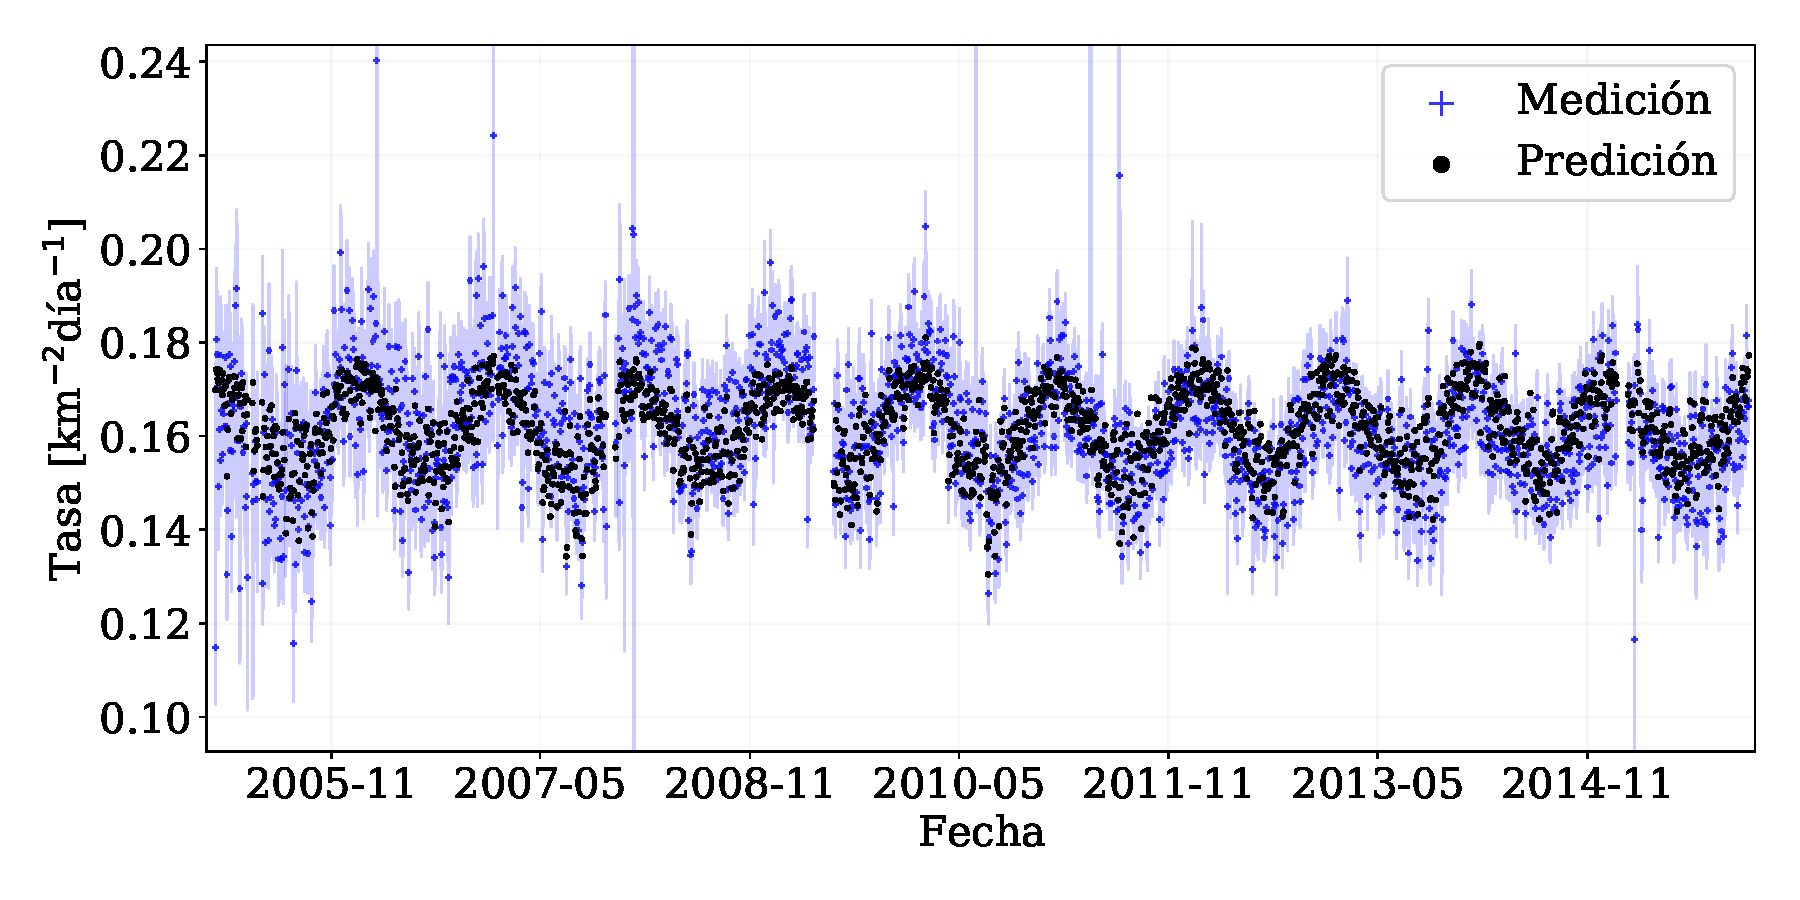
\includegraphics[width=\textwidth]{Graphs/rate_dayly/herald_old_above_1EeV_rate_day.pdf}
            \caption{Tasa eventos por día}\label{fig:rate_dayly_ICRC_2015}
            \end{subfigure}\\
            % \hspace{\fill}
            \begin{subfigure}[b]{0.9\textwidth}
            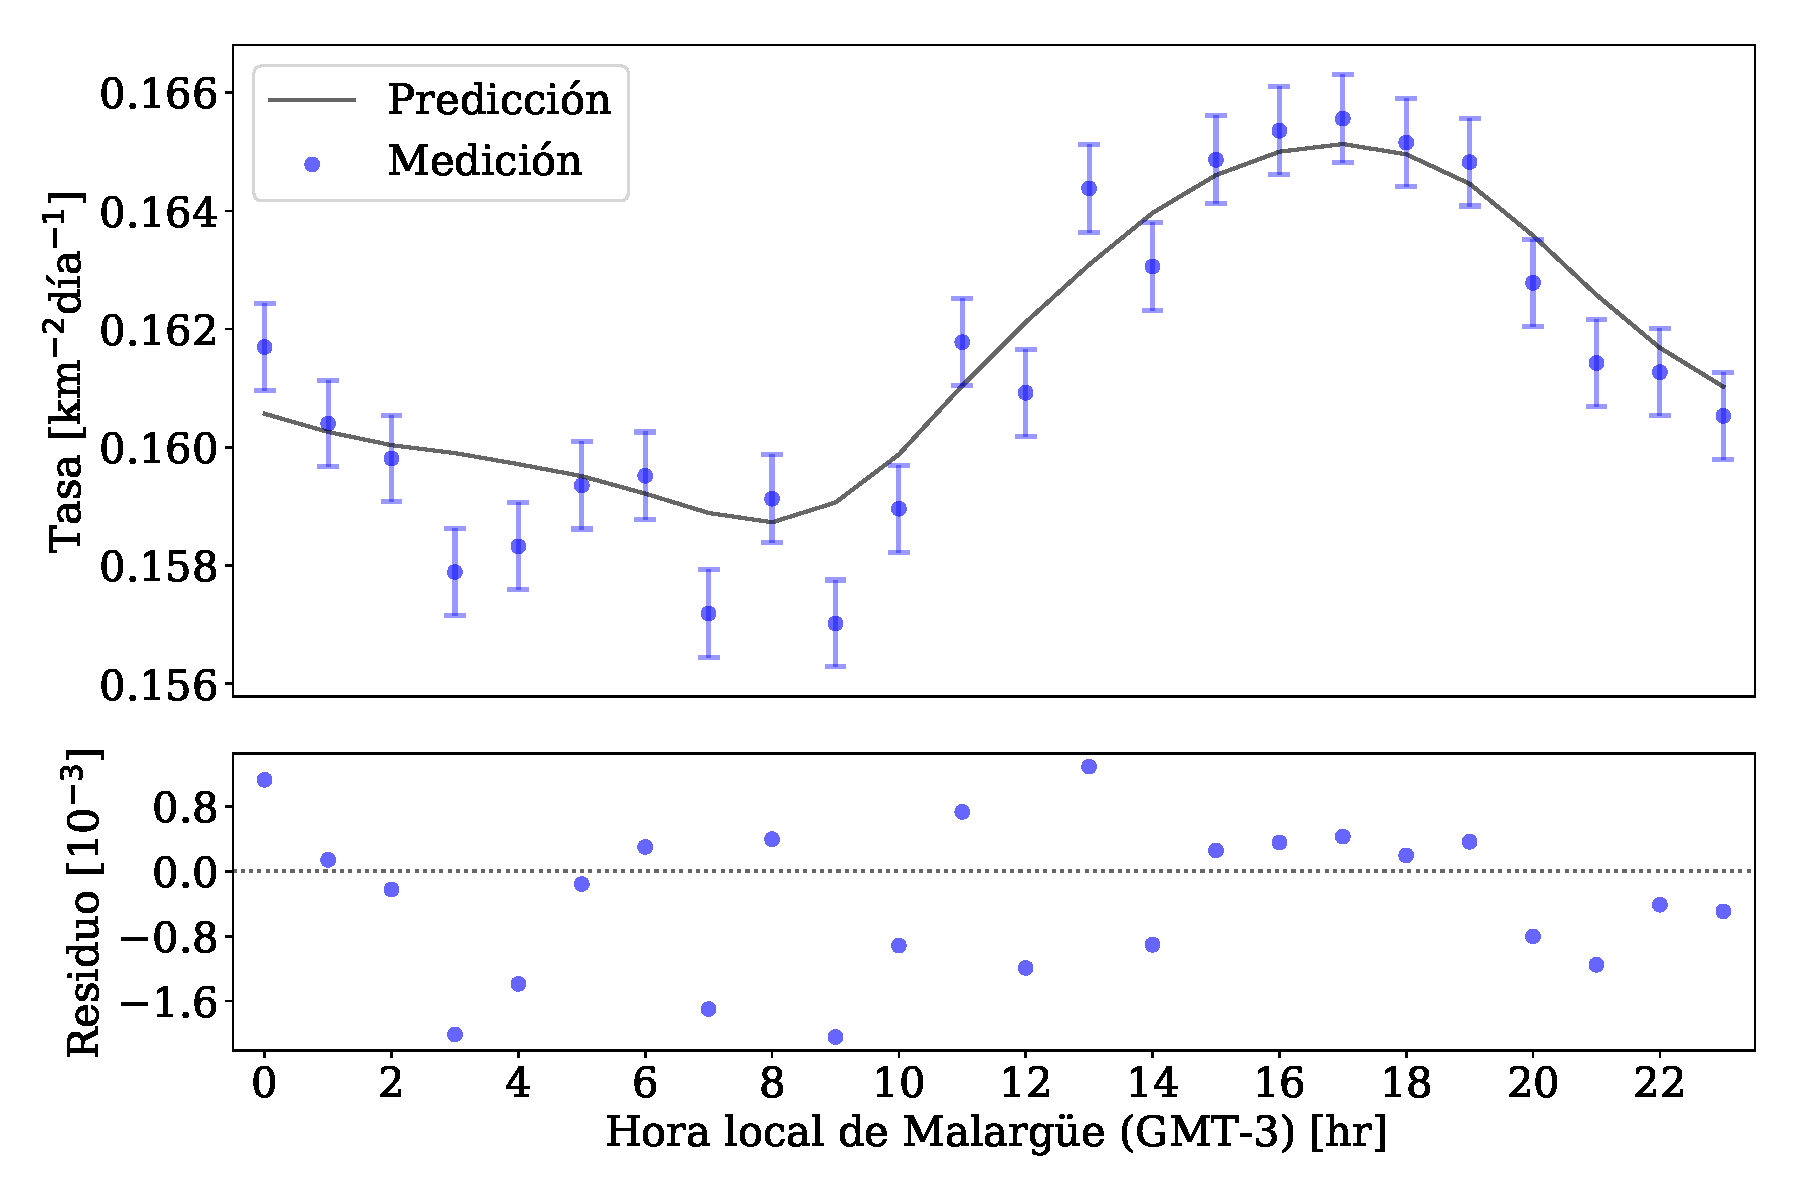
\includegraphics[width=\textwidth]{Graphs/rate_hour_of_the_day/1EeV_ICRC_2015_old_herald.pdf}
            \caption{Tasa de eventos promediada por hora del día }\label{fig:rate_hod_ICRC_2015}
            \end{subfigure}%
            \caption{Tasa de eventos por días comparadas con el ajuste entre los años 2005 hasta 2015. Los datos analizados fueron los presentados en la ICRC 2015 para energías mayores a $1\,$EeV donde se observa la modulación anual y diaria del clima. }\label{fig:rate_2015_05-15}
        \end{figure}


        Como se menciona en la sección \ref{seccion:sd_eff}, el detector alcanza su máxima eficiencia para energías mayores que 3\,EeV. A partir una energía de $2\,$EeV, los eventos tienen una mayor susceptibilidad al disparo de tres tanques, mínimo número necesario para la reconstrucción de un evento. Para el conjunto A, como se muestra en la Fig.\,\ref{fig:rate_2015_05-15_2EeV}, la modulación del clima aún es apreciable para una energía mayor a $2\,$EeV con una menor amplitud que para eventos de energía mayor a $1\,EeV$. 

        \begin{figure}[H]
            \centering
            \begin{subfigure}[b]{0.5\textwidth}
            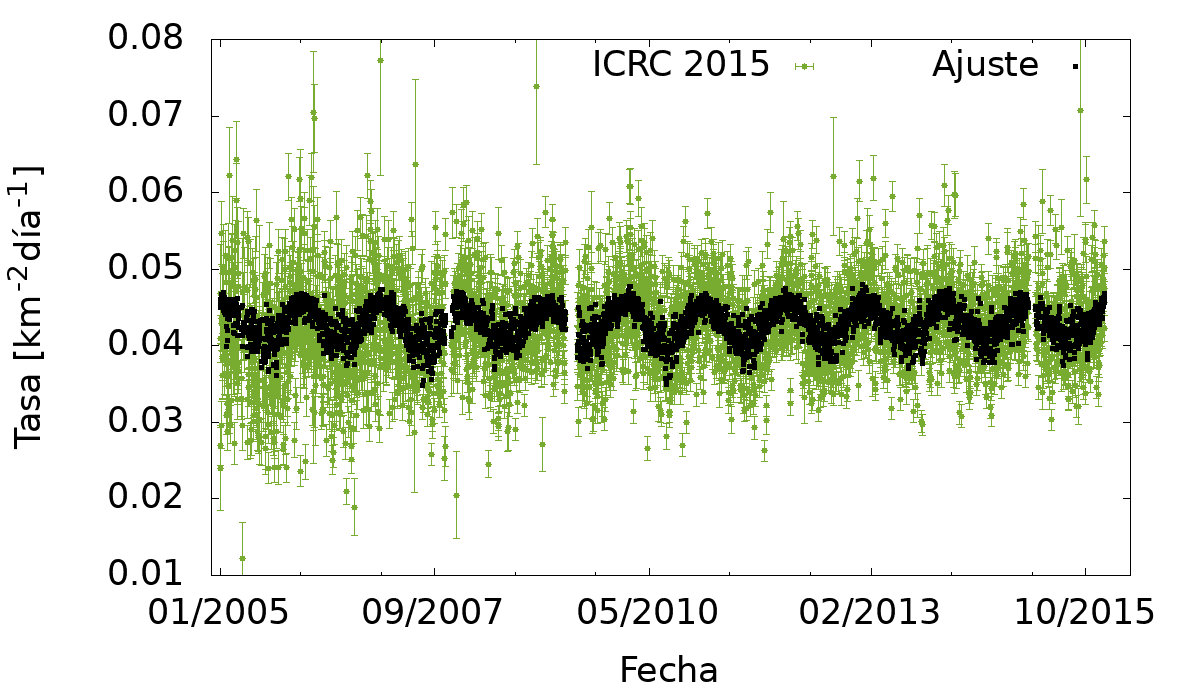
\includegraphics[width=\textwidth]{Graphs/rate_dayly/2EeV_ICRC_2015.png}
            \caption{Tasa eventos por día}\label{fig:rate_dayly_ICRC_2015_2EeV}
            \end{subfigure}\\
            % \hspace{\fill}
            \begin{subfigure}[b]{0.5\textwidth}
            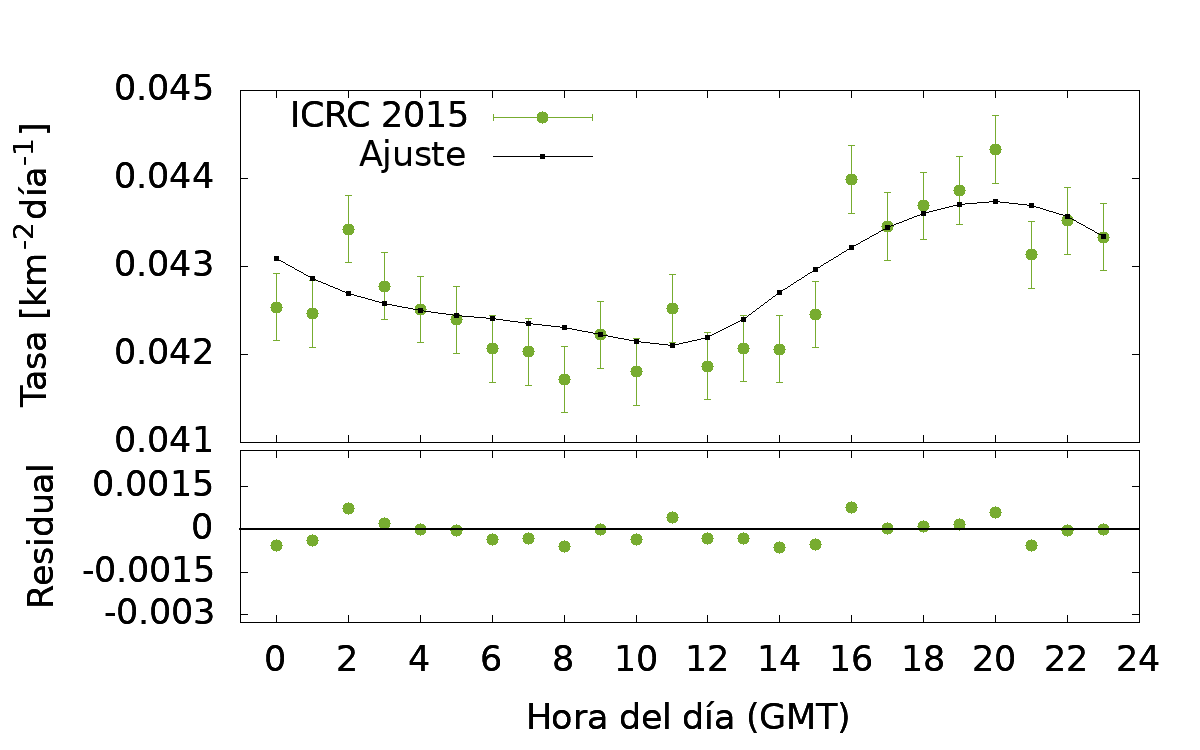
\includegraphics[width=\textwidth]{Graphs/rate_hour_of_the_day/2EeV_ICRC_2015_old_herald.png}
            \caption{Tasa de eventos promediada por hora del día }\label{fig:rate_hod_ICRC_2015_2EeV}
            \end{subfigure}%
            \caption{Tasa de eventos por días comparadas con el ajuste entre los años 2005 hasta 2015. Los datos analizados son los presentados en la ICRC 2015 para energías mayores a $2\,$EeV. donde se observa la modulación anual y diaria del clima }\label{fig:rate_2015_05-15_2EeV}
        \end{figure}

%====|====|	Weather params
        \subsubsection{Ajuste de los parámetros del clima}
        En esta sección se estudia la dependencia de los parámetros del clima con el ángulo cenital. Clasificamos los eventos en distintos subconjuntos según el valor de $sin^2(\theta)$ para realizar un ajuste análogo al presentado en la Tabla \ref{tabla:parametros_ICRC_2015}. Se clasifica mediante este valor para obtener números de eventos similares para cada subconjunto. Estos ajustes son presentados en las Figs. \ref{fig:ap_2015}, \ref{fig:arho_2015} y \ref{fig:brho_2015}. Los mismos se comparan con los datos presentados en \cite{aab2017impact}, usados actualmente en la corrección de los datos del Observatorio Pierre Auger. Se observa que los ajustes hechos sobre el conjunto A son compatibles con los ajustes realizados en  el trabajo \cite{aab2017impact}. 
%====|====|====|	ap, arho, brho 2005-2015 vs JINST over 1 EeV
                \begin{figure}[H]
                    \centering
                    \begin{subfigure}[b]{0.8\textwidth}
                    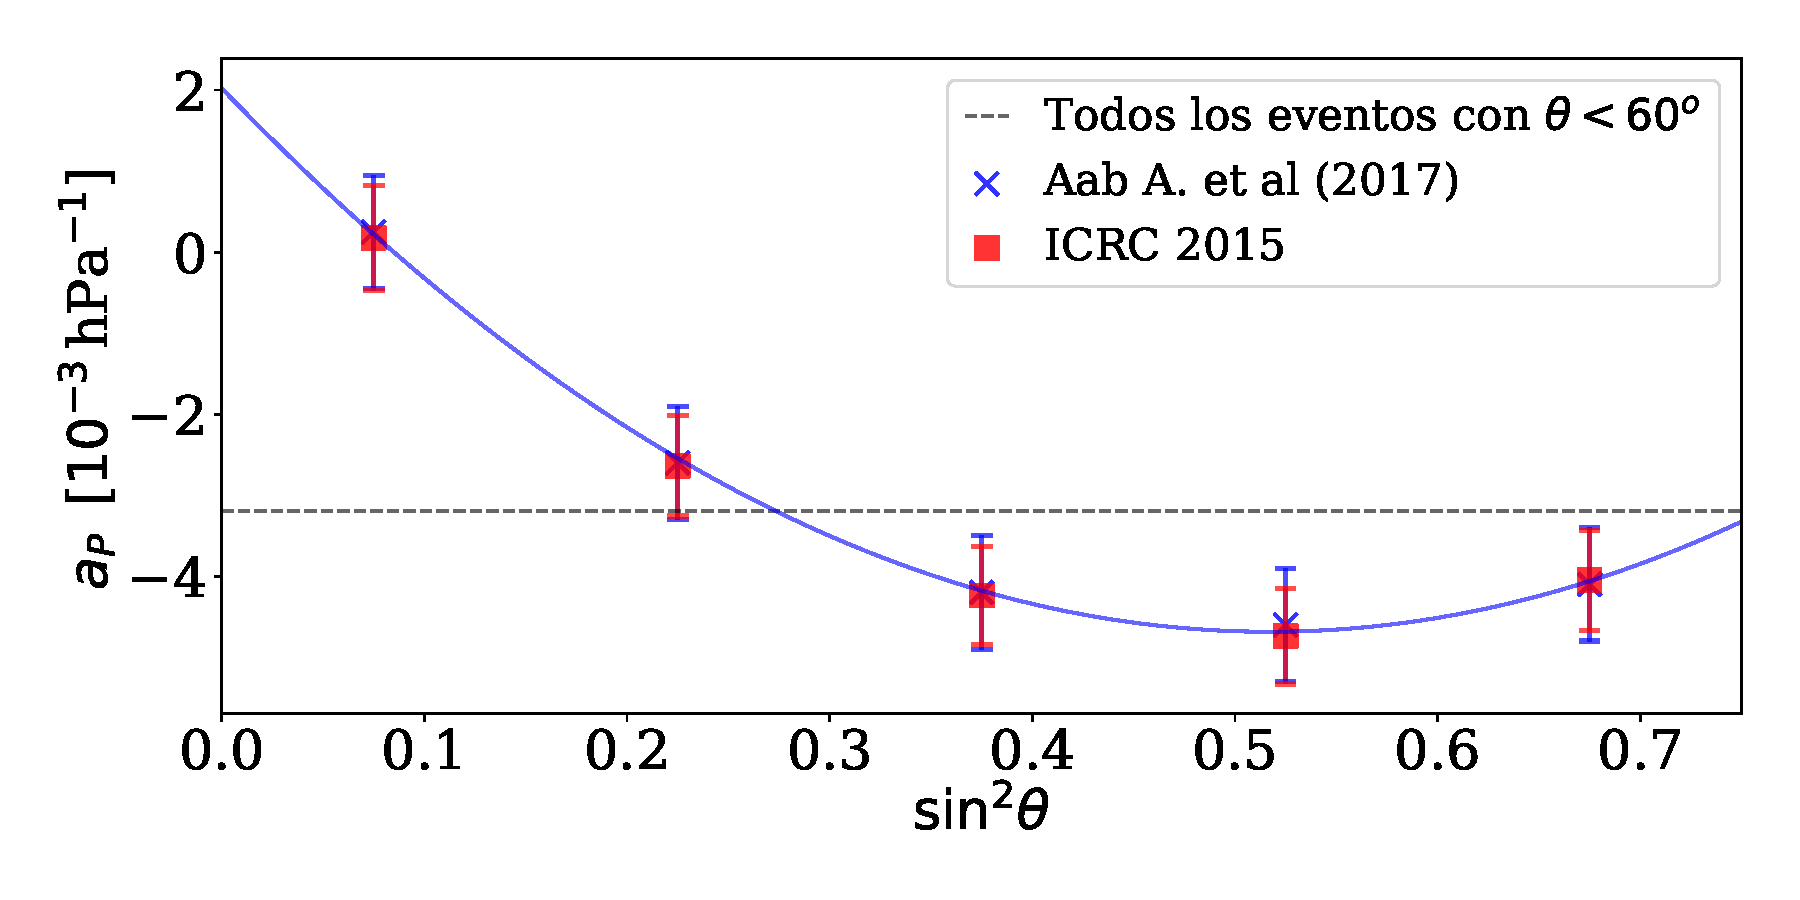
\includegraphics[width=\linewidth]{Graphs/params/ap_ICRC_2015_above_1EeV_v2.pdf}
                    \caption{Parámetro $a_P$ }
                    \label{fig:ap_2015}
                    \end{subfigure}\\
                    % \hspace{\fill}
                    \begin{subfigure}[b]{0.8\textwidth}
                    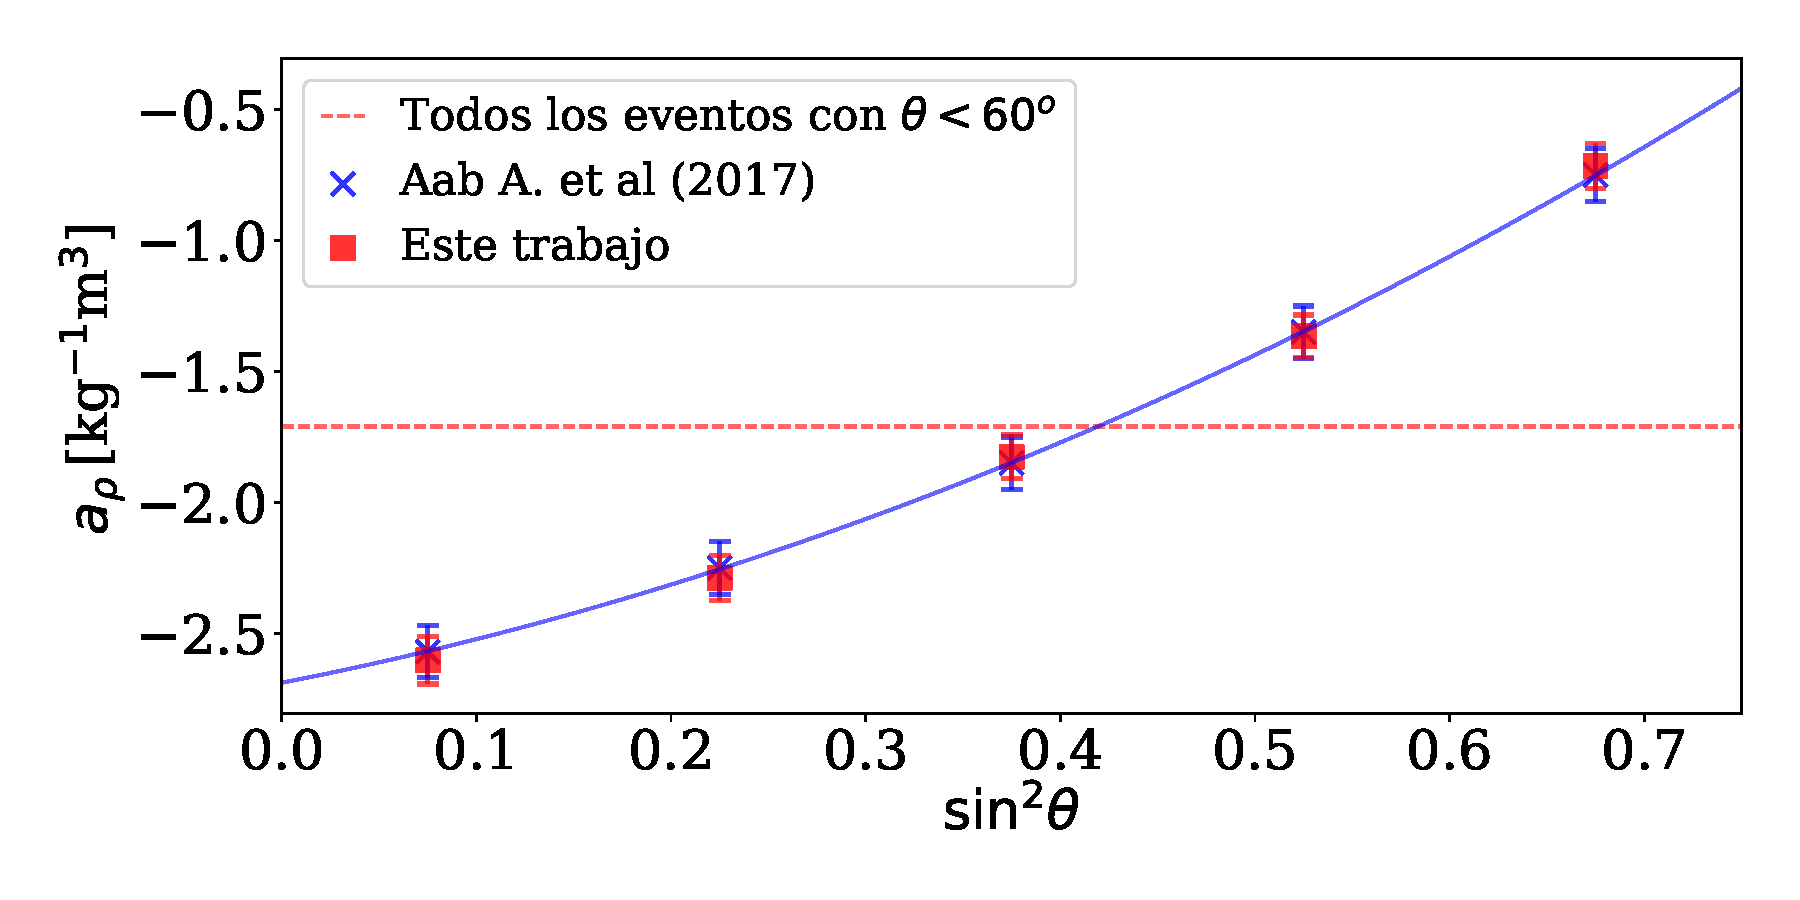
\includegraphics[width=\linewidth]{Graphs/params/arho_ICRC_2015_above_1EeV_v2.pdf}
                    \caption{Parámetro $a_{\rho}$ }
                    \label{fig:arho_2015}
                    \end{subfigure}\\
                    % \hspace{\fill}
                    \begin{subfigure}[b]{\textwidth}
                    \centering
                    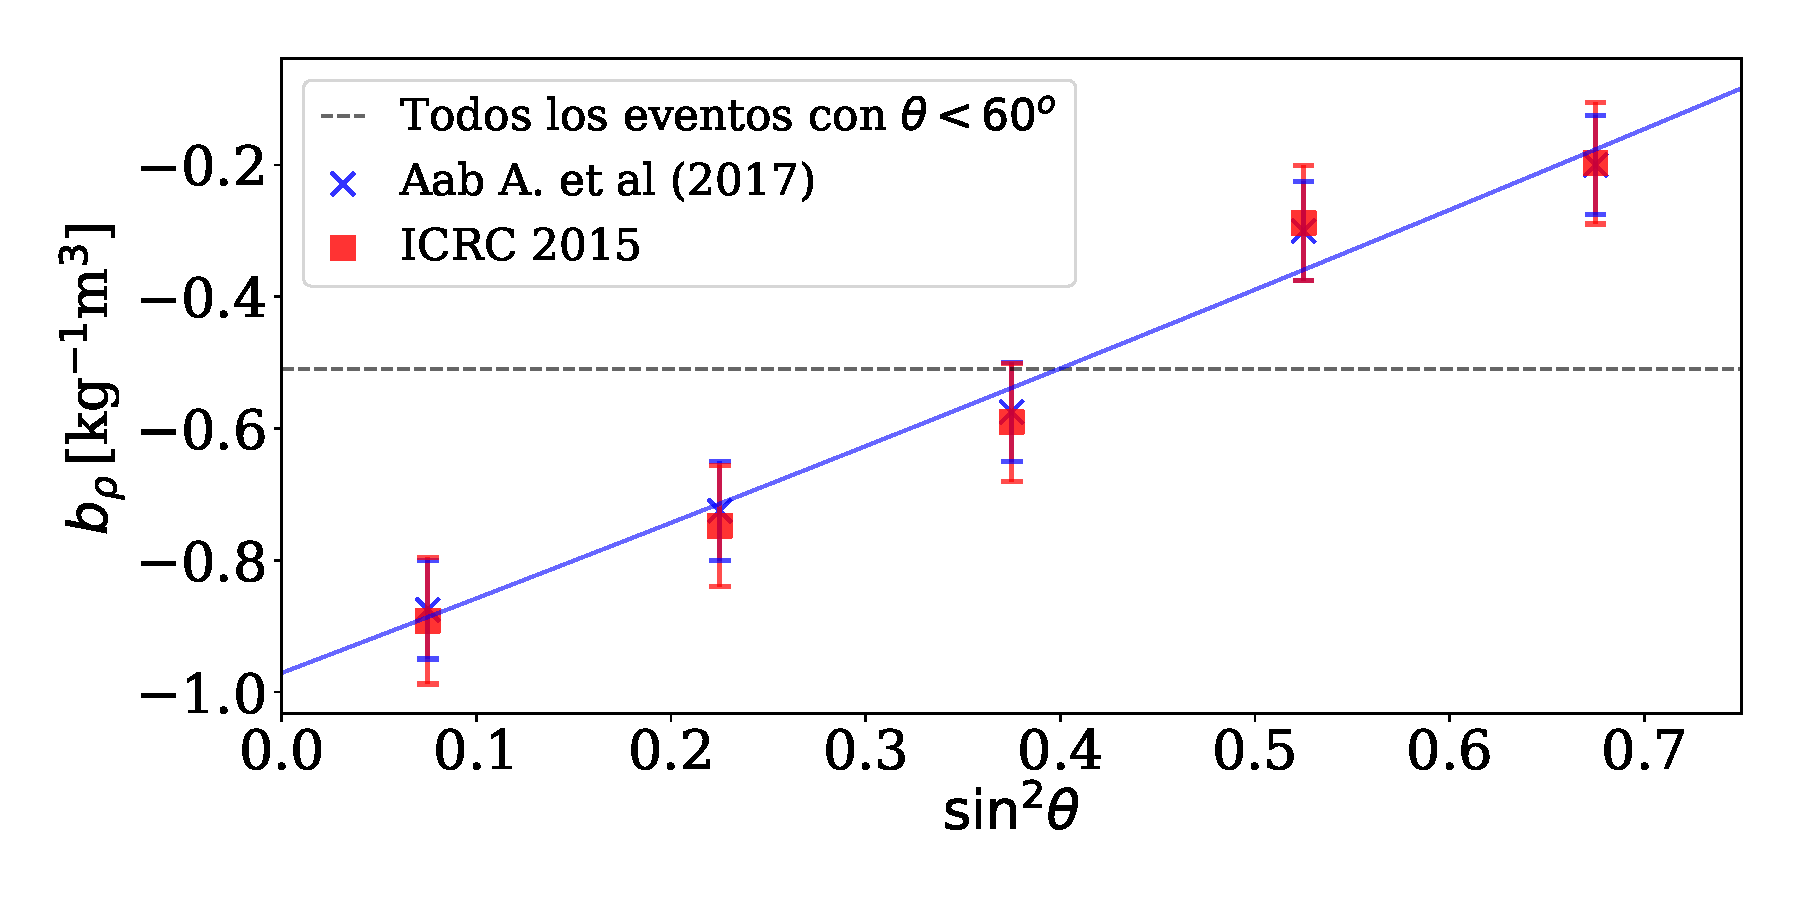
\includegraphics[width=0.8\linewidth]{Graphs/params/brho_ICRC_2015_above_1EeV_v2.pdf}
                    \caption{Parámetro  $b_{\rho}$	 }
                    \label{fig:brho_2015}
                    \end{subfigure}%
                    \caption{Parámetros de la modulación del clima considerando los datos de la ICRC 2015. Los mismos se comparan con los ajustes obtenidos por la Colaboración y con los ajustes obtenidos sin considerar la dependencia con $sin^2(\theta)$. }\label{fig:parameters_old}
                \end{figure}
%====|====|====| 	Tabla de c0, c1, c2
            En la Fig. \ref{fig:parameters_old} también se compara los ajustes obtenidos considerando los datos sin clasificar por $sin^2\theta$. Se observa que existe una dependencia con el ángulo cenital correspondiente al evento. Esta dependencia fue modelada mediante una función cuadrática dada en la Ec.\,\ref{eq:cuadratica}
            \begin{equation}
                f(x) = c_0 + c_1x + c_2x^2
                \label{eq:cuadratica}
            \end{equation}
            donde $x=sin^2\theta$.  En la Tabla\,\ref{tabla:cuadratica_ICRC_2015} se comparan los coeficientes obtenidos considerando la Ec.\,\ref{eq:cuadratica} con los mismos coeficiente obtenidos en el trabajo anterior \cite{aab2017impact}. 

        La dependencia con el ángulo cenital se debe a que para distintos ángulos de incidencia la lluvia interactúa con más o menos atmósfera. Los efectos de las condiciones climáticas afectan el desarrollo de la lluvia. Por ejemplo, el coeficiente de la presión  es negativo para $\sin^2(\theta)>0.3$ o $\theta>33^o$, lo que indica que si presión sube la señal baja. Esto es una consecuencia de que la lluvia  está en un estado más avanzado de su desarrollo. Para ángulos cenitales cercanos a $60^o$, la componente electromagnética es suprimida por las interacciones en la atmósfera, por lo tanto el efecto de la presión disminuye. El resultado obtenido en la Fig.\,\ref{fig:ap_2015} es consistente con este fenómeno, dado que el valor de $a_P$ disminuye al aumentar el ángulo. 		En el caso de los coeficientes relacionados con la densidad, también se observa que los parámetros son negativos, dado que un aumento de la densidad disminuye $r_M$ y por lo tanto la extensión de la señal. Se observa también que los parámetros $a_\rho$ y $b_\rho$ tienen la misma tendencia con $\sin^2(\theta)$, además de que los coeficientes tienen una razón de aproximadamente $\nicefrac{1}{3}$, lo cual se esperaba por lo discutido en la sección \ref{seccion:fisica_clima}.
                \begin{table}[H]
                    \centering
                    \begin{tabular}{l|l|l|l}\hline
                         Parámetros									& Coeficiente		& Este Trabajo			& \cite{aab2017impact}	\\ \hline
                     \multirow{3}{*}{$a_P$ [hPa$^{-1}$]}  			&  $c_0$			& $( 2.00\pm 0.05)\times 10^{-3}$	& $( 2.1 \pm 0.9)\times 10^{-3} $	\\ \cline{2-4} %Done
                                                                    &  $c_1$			& $(-26.3 \pm 0.2)\times 10^{-3}$	& $(-26.0 \pm 0.6 )\times 10^{-3}$	\\ \cline{2-4} 
                                                                    &  $c_2$			& $( 25.7 \pm 0.2)\times 10^{-3}$	& $( 26.0 \pm 0.7 )\times 10^{-3}$	\\ \hline % 
                    
                     \multirow{3}{*}{$a_\rho$ [kg$^{-1}$m$^3$]}  	&  $c_0$			& $-2.73   \pm 0.05$	& $ -2.7  \pm 0.1  $\\ \cline{2-4} 
                                                                    &  $c_1$			& $ 1.5    \pm 0.4 $	& $ 1.5   \pm 0.8  $\\ \cline{2-4} 
                                                                    &  $c_2$			& $ 2.1    \pm 0.7 $	& $ 2.2   \pm 1.0  $\\ \hline %
                    
                    \multirow{3}{*}{$b_\rho$ [kg$^{-1}$m$^3$]} 		&  $c_0$			& $-1.0    \pm 0.1$		& $-1.0   \pm 0.1 $	\\ \cline{2-4} 
                                                                    &  $c_1$			& $ 1.2    \pm 0.6$		& $ 1.2   \pm 0.8  $	\\ \cline{2-4} 
                                                                    &  $c_2$			& $ 0.1    \pm 0.8$		& $ 0.0   \pm 1.1  $	\\ 
                    
                    \end{tabular}	
                    \caption{Tabla de los coeficientes obtenidos para el conjunto de datos de la ICRC 2015, comparados con los parámetros de la reconstrucción de los eventos del Observatorio.} \label{tabla:cuadratica_ICRC_2015}
                \end{table}

%==================================================================================
%==================================================================================
%==================================================================================
%==================================================================================

%====|==> ICRC 2019
 \subsection{Datos presentados en la ICRC 2019}\label{conjuntoB}

     Comparando este conjunto de datos con los datos de la ICRC 2015, los datos de la ICRC 2019 contienen eventos de los tres años posteriores. Posterior al trabajo \cite{aab2017impact}, la señal de S(1000) fue corregida por las condiciones climáticas en la reconstrucción oficial de eventos. Además el valor de S(1000) estimado para cada evento cambió entre estos dos conjuntos de datos, por parte de la reconstrucción oficial \cite{isabel}. Se realizó también una nueva calibración de la energía mediante eventos híbridos, como la mostrada en la Fig.\,\ref{fig:efd_s38} en el trabajo  \cite{tobepublished}. 
     
     En el conjunto de datos de la ICRC 2019, se realizó los mismos cortes que para el conjunto de A de la sección anterior. En el periodo 2005-2015 de los datos de la ICRC 2019 con los cortes mencionados de energía mayor a $1\,$EeV para eventos verticales, la cantidad de eventos con energías mayores a $1\,$EeV subió de $1\,146\,470$ a  $1\,280\,918$ eventos. Esto puede deberse a la corrección del clima de los eventos, donde aquellos eventos que estaban por debajo del corte del energía, tras la corrección pudieron estar por encima de este corte. Otra posibilidad es que la nueva reconstrucción haya aumentado la cantidad de eventos por encima de $1\,$EeV, por eso la energía media bajó de $2.00\,$EeV a $1.91\,$EeV.  Las características de los datos en los rangos de tiempo relevantes se resumen en la Tabla\,\ref{tabla:caracteristicas_ICRC_2019}. 

%====|====|	Tabla de eventos exposure
        \begin{table}[H]
            \centering
            \begin{tabular}{|c|c|c|}
            {Tiempo }           & {01/01/2005-31/12/2015}   & {01/01/2005-31/12/2018 }\\ \hline 
            Número de eventos   &  1280918     			    &  1635045     		        \\ \hline 
            Energía media       &  1.91				        &	1.92				        \\ \hline 
            Corte en energía    &  1 EeV       		 	    &  1 EeV       		 \\ \hline 
            Corte en ángulo cenital	&  $60^o$ 				    & $60^o$\\ 
            \end{tabular}
            \caption{Características de los datos de la ICRC 2019 utilizados para los ajustes de esta sección.} \label{tabla:caracteristicas_ICRC_2019}
        \end{table}

        En la Fig.\,\ref{fig:rate_new_18} se muestran las tasas de eventos por día para energía mayores a $1\,$EeV y $2\,$EeV, con la energía corregida por los efectos climáticos según la reconstrucción oficial \cite{data}. En la Fig.\,\ref{fig:rate_new_18_2EeV} se  comparan con los resultados de los datos de la ICRC 2015, la modulación en la tasa ya no es apreciable. Si comparamos las tasas de eventos por hora del día de los eventos por encima de $1\,$EeV y $2\,$EeV, por encima de $1\,$EeV, se aprecia un remanente de la modulación del clima diaria comparado con la tasa para $2\,$EeV. Esto se debe a que el SD tiene eficiencia para energía mayores a $3\,$EeV, comentado anteriormente.


        Existe una modulación remanente en la tasa de eventos como se aprecia en las Figs.\,\ref{fig:rate_day_ICRC_19_05_18} y \ref{fig:rate_day_ICRC_19_05_18_2EeV}. Esto se debe que la señal es mayor que la esperada como consecuencia de las condiciones atmosféricas en el momento del evento, por lo tanto la eficiencia del disparo ante este evento también es mayor. De esta forma la eficiencia tiene una dependencia con las condiciones atmosféricas.

%====|====|	2005-2019	rate day over 1 EeV
%====|====|	2005-2019	rate hour of the day	1 EeV
        \begin{figure}[H]
            \centering
            \begin{subfigure}[b]{0.5\textwidth}
            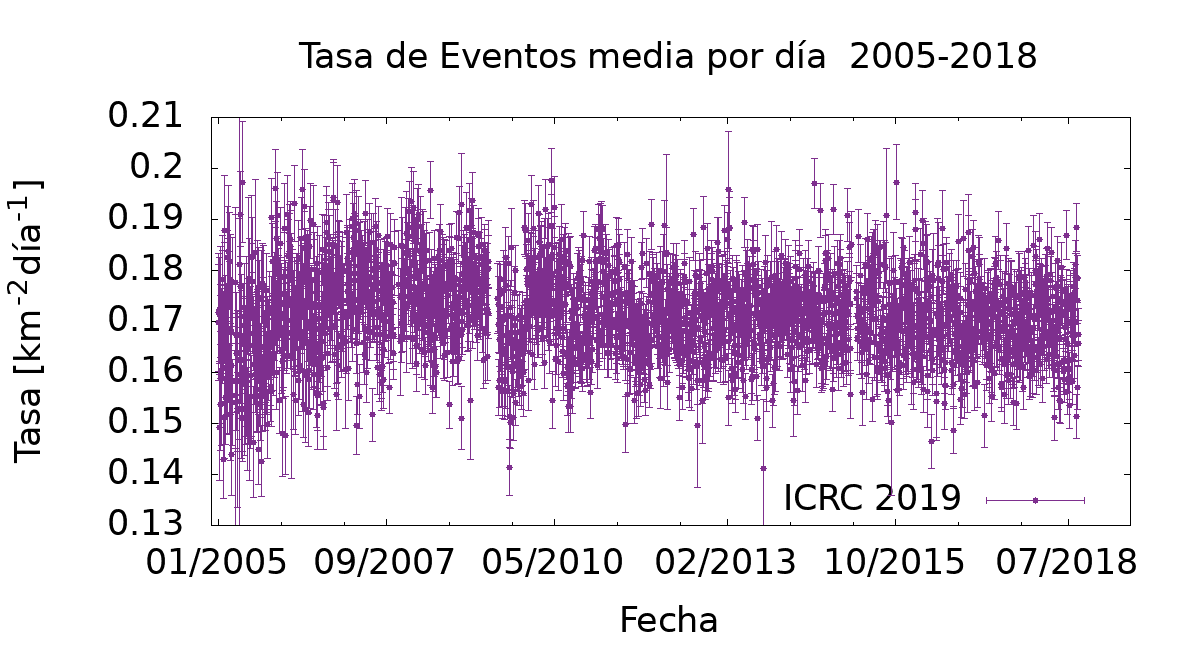
\includegraphics[width=\textwidth]{Graphs/rate_dayly/1EeV_ICRC_2019_05_18.png}
            \caption{Energía mayor a $1\,$EeV}
            \label{fig:rate_day_ICRC_19_05_18}
            \end{subfigure}\\
            % \hspace{\fill}
            \begin{subfigure}[b]{0.5\textwidth}
            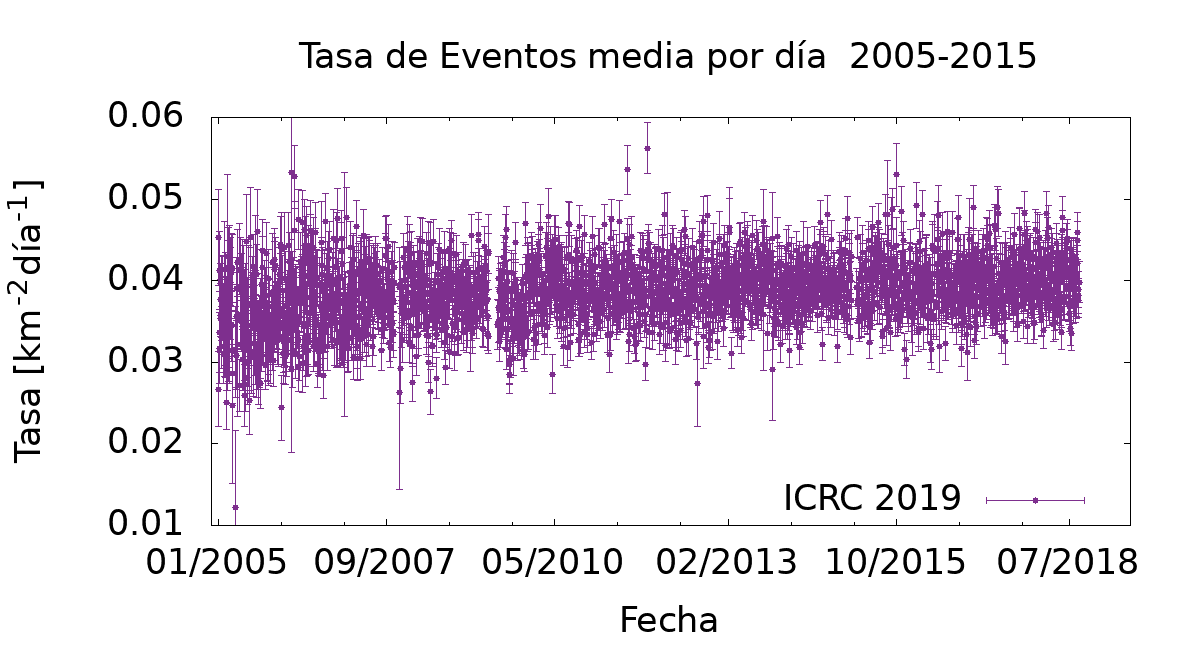
\includegraphics[width=\textwidth]{Graphs/rate_dayly/2EeV_ICRC_2019_05_19.png}
            \caption{ Energía mayor a $2\,$EeV}
            \label{fig:rate_2015_ICRC_19_05_18}
            \end{subfigure}%
            \caption{Tasa de eventos promedio por cada día entre los años 2005 hasta 2015 del conjunto de datos presentado en la ICRC 2019. Se muestran las tasas para dos cortes en energía, mayor a $1\,$EeV y mayor a $2\,$EeV}\label{fig:rate_new_18}
        \end{figure}
        \begin{figure}[H]
            \centering
            \begin{subfigure}[b]{0.495\textwidth}
            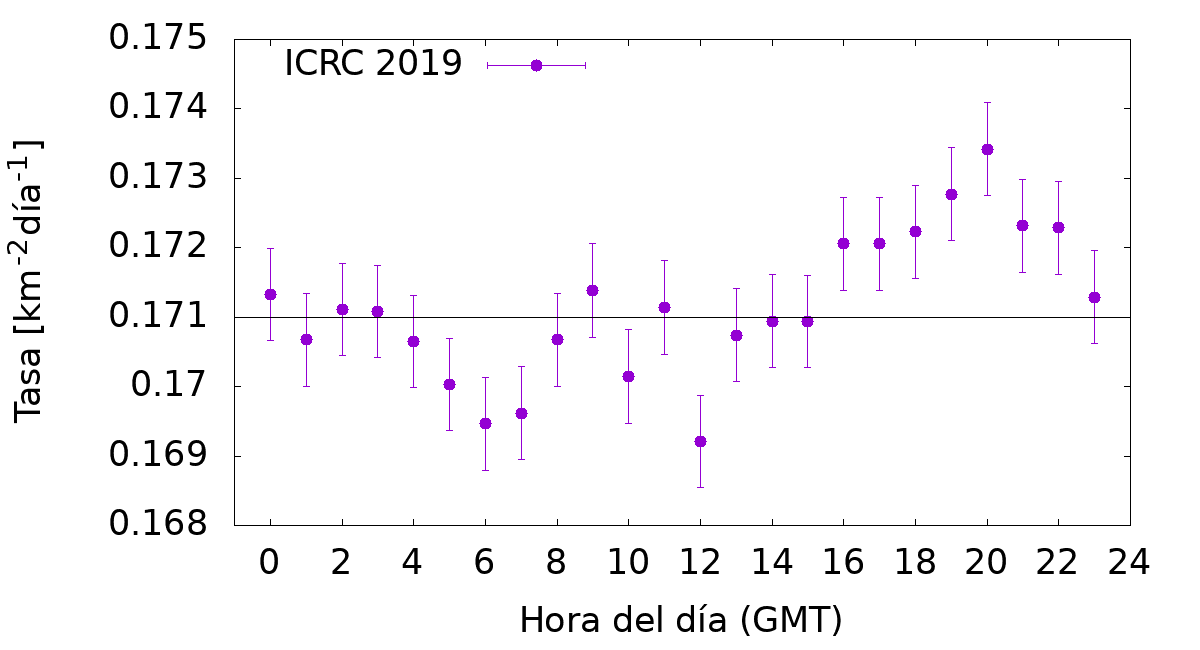
\includegraphics[width=\textwidth]{Graphs/rate_hour_of_the_day/1EeV_ICRC_2019_05_19.png}
            \caption{Energía mayor a $1\,$EeV}
            \label{fig:rate_day_ICRC_19_05_18_2EeV}
            \end{subfigure}\\
            % \hspace{\fill}
            \centering
            \begin{subfigure}[b]{0.495\textwidth}
            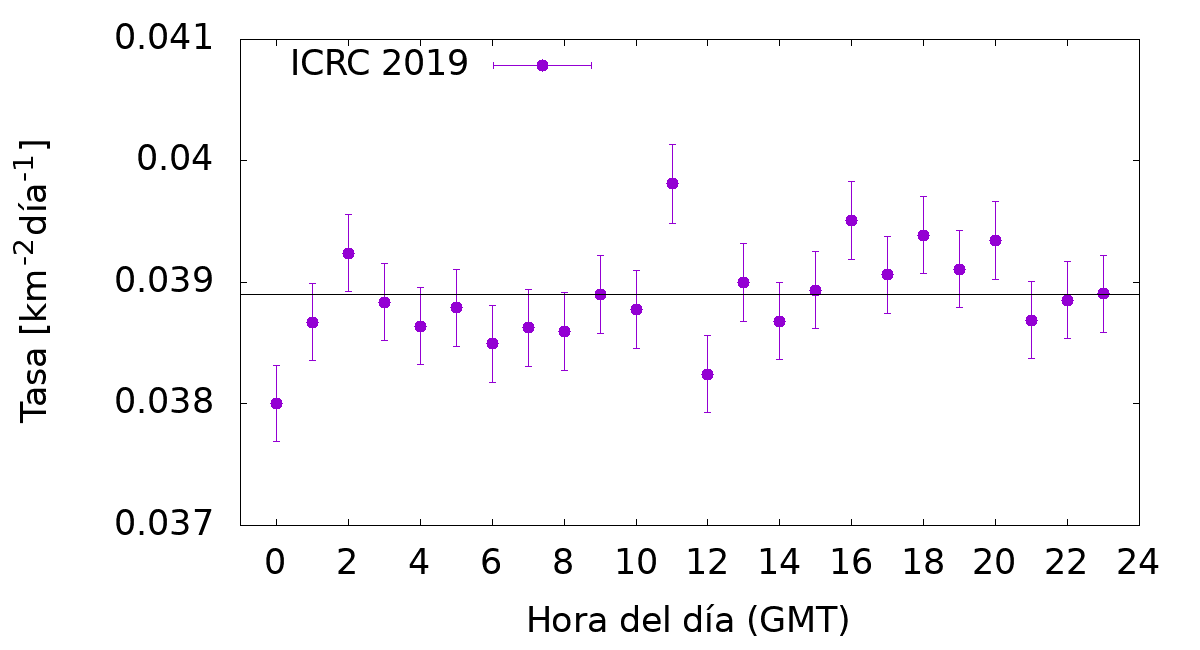
\includegraphics[width=\textwidth]{Graphs/rate_hour_of_the_day/2EeV_ICRC_2019_05_18.png}
            \caption{Energía mayor a $2\,$EeV}
            \label{fig:rate_2015_ICRC_19_05_18_2EeV}
            \end{subfigure}%
            \caption{Tasa eventos  por hora del día por unidad de área entre los años 2005 hasta 2015 del conjunto de datos presentado en la ICRC 2019.  Se muestran las tasas para dos cortes en energía, mayor a $1\,$EeV y mayor a $2\,$EeV}\label{fig:rate_new_18_2EeV}
        \end{figure}



%====|==>ICRC 2019 S$_{38}$-Sin Corrección
\subsection{Datos presentados en la ICRC 2019 usando $S_{38}$ sin corregir por el clima} \label{sin_corregir_s38}

Además de tener más estadística de los eventos registrados, durante el periodo 2016-2018 también se recabaron datos sobre el clima en el observatorio. En la modulación del clima estudiada con el conjunto A, se  realiza un corte de la energía sin corregir. En esta sección se realiza el análisis de la modulación mediante un  corte sobre la señal medida por el SD. En el conjunto de datos de la ICRC 2019, es posible acceder al valor de S(1000) sin corregir por el trabajo \cite{aab2017impact}, por lo que uno puede obtener el valor de S$_{38}$ sin corregir mediante la expresión
\begin{equation}
    S_{38} = \frac{S(1000)}{S(1000)_w}S_{38,w}
    \label{eq:s38_w}
\end{equation}
donde las variables $S(1000)_w$ y $S_{38,w}$ indican los valores corregidos por clima. Estas variables están listadas en el conjunto de datos presentado en la ICRC 2019. Dado que los trabajos anteriores se basaron en la energía para hacer el corte de los eventos, se realizó el corte con la señal de $S_{38}\ge 5.37\,$VEM correspondiente a 1\,EeV aproximadamente. Las características de este conjunto de datos están resumidos en la Tabla\,\ref{tabla:caracteristicas_ICRC_2019_S38}.
%====|====|	Tabla de eventos exposure
        \begin{table}[H]
            \centering
            \begin{tabular}{c|c|c}
            {Tiempo}                & {01/01/2005-31/12/2015}   & {01/01/2005-31/12/2018 }\\ \hline 
            Número de eventos       &   $1\,267\,265$     	    &  $1\,618\,717$     		\\ \hline 
            Energía media           &  1.89        		 	    &  1.90        		\\ \hline 
            Corte en S$_{38}$ 	    &  5.37\,VEM   		 	    &  5.37\,VEM       	\\ \hline 
            Corte en ángulo cenital &  $<60^o$ 			 	 & $<60^o$\\ 
            \end{tabular}
            \caption{Características de los datos de la ICRC 2019 utilizados para los ajustes de esta sección.} \label{tabla:caracteristicas_ICRC_2019_S38}
        \end{table}
        
%====|====| Tabla del fit
        Con estos eventos, se realizó un  ajuste de los parámetros del clima para todos los ángulos cenitales de la tasa del eventos por hora. Así se obtienen los coeficientes promediados por ángulo cenital. Estos parámetros son presentados en la Tabla\,\ref{tabla:parametros_ICRC_2019_S38}. Se observa que para ambos periodos estudiados los parámetros obtenidos son compatibles entre sí, además de ser compatibles con los resultados obtenidos para el periodo 2005-2015 de los datos de la ICRC 2015 y los parámetros de \cite{aab2017impact}, presentados en la Tabla\,\ref{tabla:parametros_ICRC_2015}.

        \begin{table}[H]
            \centering
            \begin{tabular}{|c|c|c|}
            \hline
            {Parámetro}                 & {2005-2015}    		        & {2005-2018}    \\ \hline
            $a_P$ [hPa$^{-1}$]          & $ (-3.3\pm 0.3)\times 10^{-3}$& $(-3.2\pm 0.2)\times 10^{-3}$  \\ \hline
            $a_\rho$ [kg$^{-1}$m$^3$]   & $ -1.75\pm 0.04$            	& $ -1.71\pm 0.03$       \\ \hline
            $b_\rho$ [kg$^{-1}$m$^3$]   & $ -0.51\pm 0.04$             	& $ -0.52\pm 0.03$       \\ \hline
            $\chi^2_\nu$                & $1.00616$                     & $1.01819$              \\   \hline
            \end{tabular} 
            \caption{Parámetros del clima obtenidos para todos los ángulos cenitales para los dos rangos de tiempo estudiados.} \label{tabla:parametros_ICRC_2019_S38}
        \end{table}
        
        Calculando la tasa de eventos esperado con los parámetros de la Tabla\,\ref{tabla:parametros_ICRC_2019_S38}, esta se comparan con la tasa experimental medida con el SD, que se muestra en la Fig. \ref{fig:rate_new_18_S38} para el rango de tiempo 2005-2018. En estos gráficos se observa que la modulación del clima tiene la mismas características que las observadas en la sección \ref{icrc2015}.

        \begin{figure}[H]
            \begin{subfigure}[b]{0.5\textwidth}
            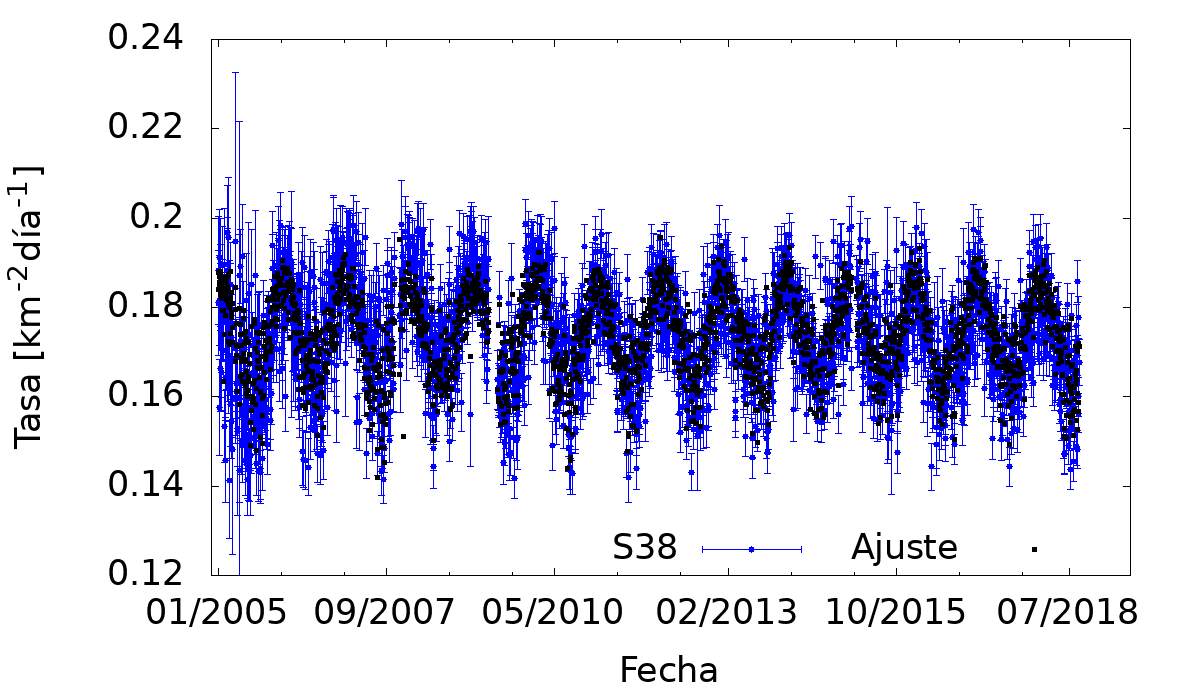
\includegraphics[width=\textwidth]{Graphs/rate_dayly/0EeV_ICRC_2019_S38_05_18.png}
            \caption{Tasa eventos por cada día por unidad de área}
            \label{fig:rate_day_ICRC_19_S38_05_18}
            \end{subfigure}%
            \hspace{\fill}
            \begin{subfigure}[b]{0.5\textwidth}
            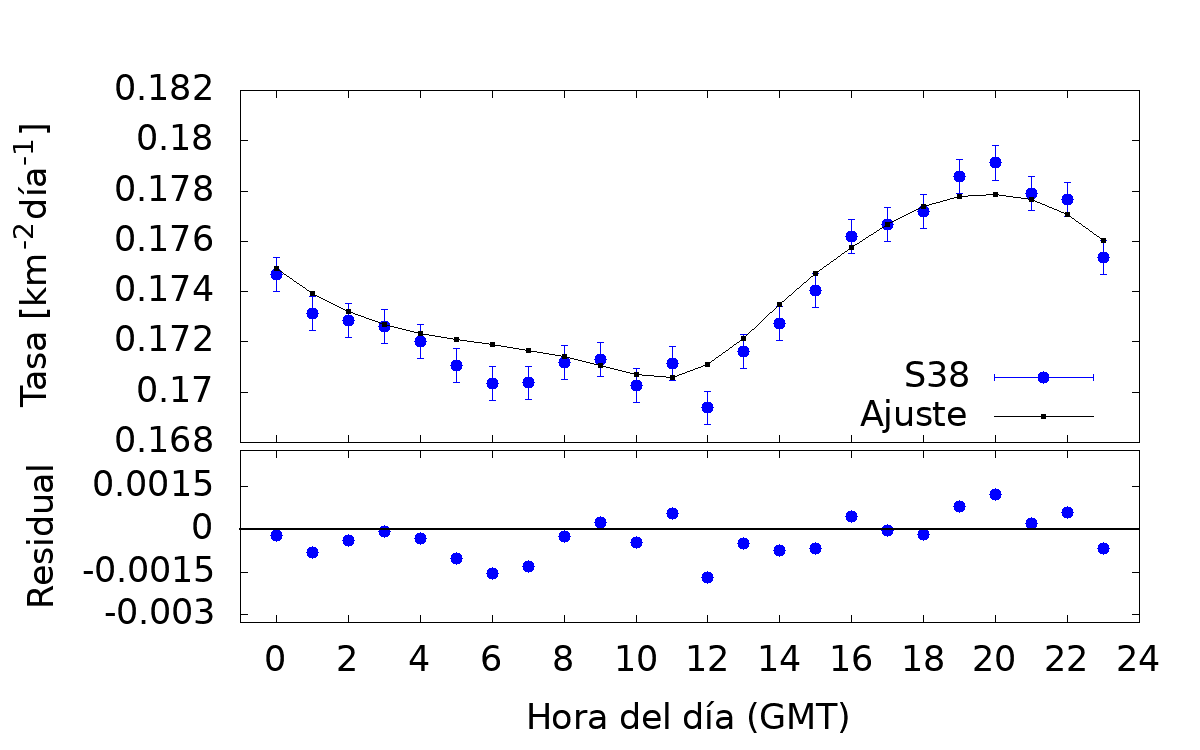
\includegraphics[width=\textwidth]{Graphs/rate_hour_of_the_day/0EeV_ICRC_2019_S38_05_18.png}
            \caption{Tasa de eventos promedio por hora del día}
            \label{fig:rate_2015_ICRC_19_S38_05_18}
            \end{subfigure}%
            \caption{Tasa de eventos entre los años 2005 hasta 2018 del conjunto de datos presentado en la ICRC 2019.}\label{fig:rate_new_18_S38}
        \end{figure}

%====|====|	Weather params
    \subsubsection{Ajuste de los parámetros del clima}

    En esta sección se clasificó los eventos mediante el valor de $sin^2\theta$ y se realizó el ajuste para obtener los parámetros del clima. Este ajuste se realizó en el periodo 2005-2018. Los valores obtenidos se resumen en la Tabla\,\ref{tabla:cuadratica_ICRC_2019_S38} y se  observan en la Fig.\,\ref{fig:parameters_new_S38}. Comparando estos resultados con los resultados de \cite{aab2017impact}, los eventos mediante el valor S$_{38}$  conservan la tendencia con $sin^2\theta$ que se observa en los datos de la ICRC 2015 en la Fig.\,\ref{fig:parameters_old}. Además los parámetros obtenidos mediante el corte por S$_{38}$ son comparables con los resultados obtenidos para el conjunto de datos de la ICRC 2015. Por lo que puede decirse que la modulación del clima es apreciable  hasta el día de hoy con una amplitud comparable al año 2015.

%====|====|====| ap, arho, brho 2005-2015  2005-2019 vs JINST over 1 EeV
            \begin{figure}[H]
                \begin{subfigure}[b]{0.5\textwidth}
                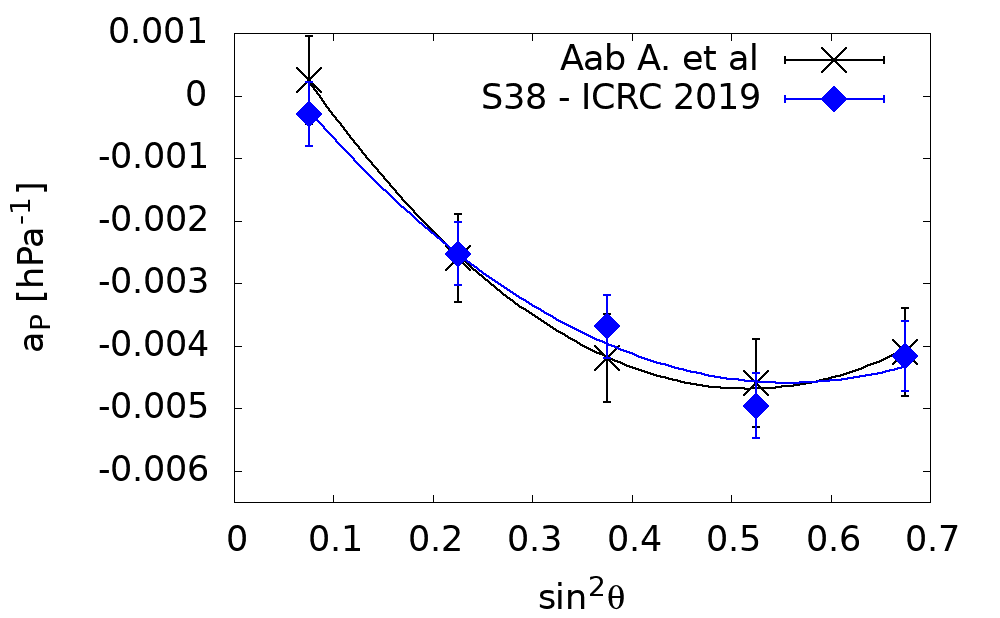
\includegraphics[width=\linewidth]{Graphs/params/ap_ICRC_2019_S38_above_0EeV.png}
                \caption{Parámetro $a_P$ }
                \label{fig:ap_2019_S38}
                \end{subfigure}%
                \hspace{\fill}
                \begin{subfigure}[b]{0.5\textwidth}
                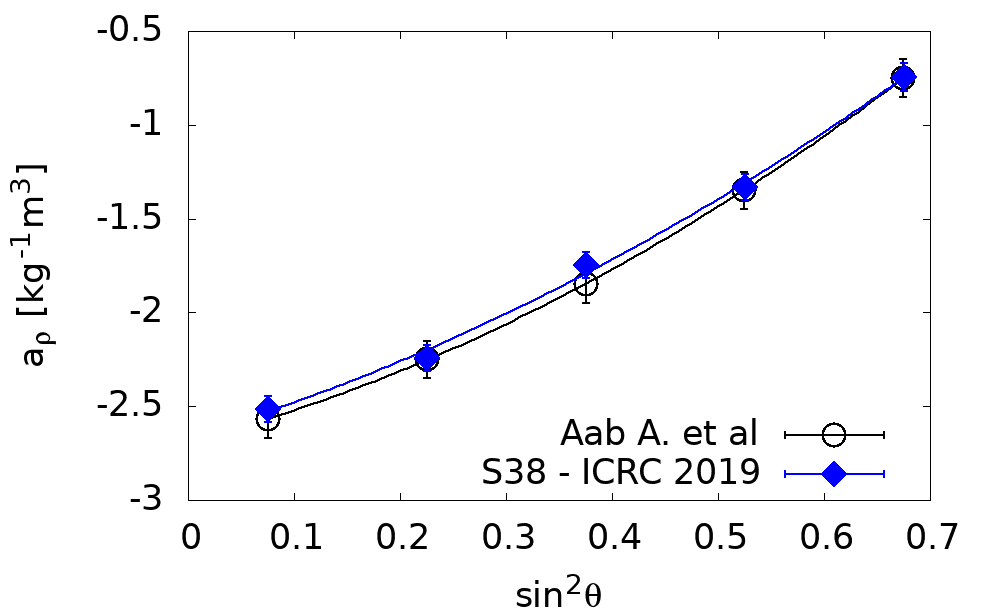
\includegraphics[width=\linewidth]{Graphs/params/arho_ICRC_2019_S38_above_0EeV.png}
                \caption{Parámetro $a_{\rho}$ }
                \label{fig:arho_2019_S38}
                \end{subfigure}%
                \hspace{\fill}
                \begin{subfigure}[b]{\textwidth}
                \centering
                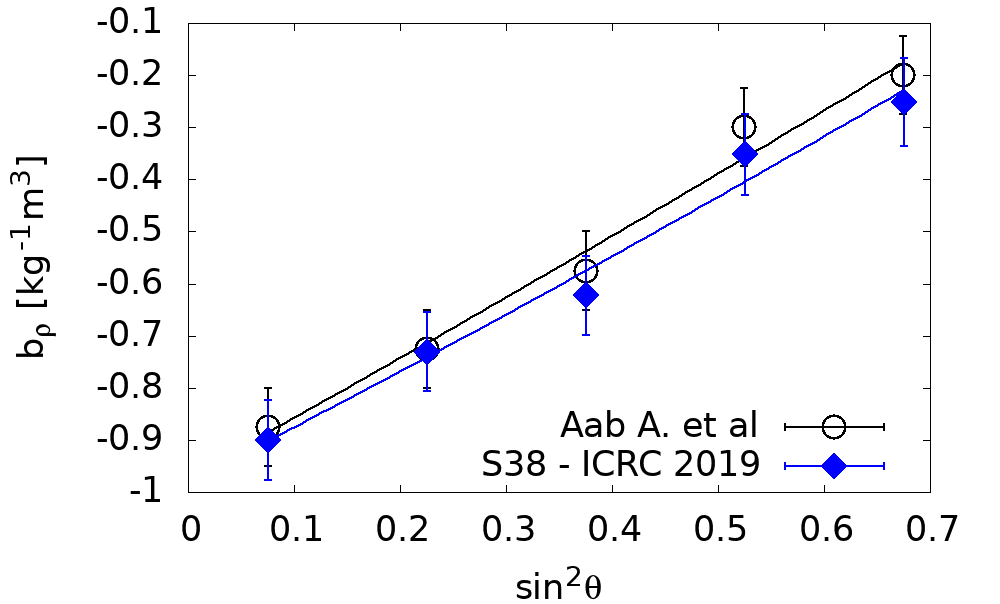
\includegraphics[width=0.5\linewidth]{Graphs/params/brho_ICRC_2019_S38_above_0EeV.png}
                \caption{Parámetro  $b_{\rho}$	 }
                \label{fig:brho_2019_S38}
                \end{subfigure}%
                \caption{Parámetros de la modulación del clima considerando los datos sin corregir con el clima y la reconstrucción anterior.}\label{fig:parameters_new_S38}
            \end{figure}
%====|====|====| Tabla de c0, c1, c2
                \begin{table}[H]
                    \centering
                    \begin{tabular}{|l|l|l|l|}\hline
                     \textbf{Parámetros}						& \textbf{Coeficiente}	& \textbf{Este Trabajo} & Reportado por \textbf{ \cite{aab2017impact}}	\\ \hline
                     \multirow{3}{*}{$a_P$ [hPa$^{-1}$]}  		&  $c_0$				& $ (0.12\pm0.05)\times 10^{-3}$	    & $(2.1 \pm 0.09)\times 10^{-3} $	\\ \cline{2-4} %Done
                                                                &  $c_1$				& $ (-2.0\pm0.3)\times 10^{-3}$		& $(-2.6  \pm 0.6)\times 10^{-3} $	\\ \cline{2-4} 
                                                                &  $c_2$				& $ (1.9\pm0.4)\times 10^{-3}$		& $(2.6   \pm 0.7)\times 10^{-3} $	\\ \hline % 
                    
                     \multirow{3}{*}{$a_\rho$ [kg$^{-1}$m$^3$]} &  $c_0$			& $-2.66   \pm 0.07$	& $ -2.7  \pm 0.1  $\\ \cline{2-4} 
                                                                 &  $c_1$			& $ 1.7    \pm 0.4 $	& $ 1.5   \pm 0.8  $\\ \cline{2-4} 
                                                                &  $c_2$			& $ 1.7    \pm 0.6 $	& $ 2.2   \pm 1.0  $\\ \hline %
                    
                    \multirow{3}{*}{$b_\rho$ [kg$^{-1}$m$^3$]} 	&  $c_0$			& $-0.98    \pm 0.08$	& $-1.0   \pm 0.1 $	\\ \cline{2-4} 
                                                                &  $c_1$			& $ 1.00    \pm 0.5$	& $ 1.2   \pm 0.8  $	\\ \cline{2-4} 
                                                                &  $c_2$			& $ 0.1    \pm 0.6$		& $ 0.0   \pm 1.1  $	\\ \hline 
                    
                    \end{tabular}	
                    \caption{Tabla de los coeficientes obtenidos con el S$_{38}$ sin corregir por el clima, comparados con el trabajo anterior} \label{tabla:cuadratica_ICRC_2019_S38}
                \end{table}

%=================================================================================
%=================================================================================
%=================================================================================
%=================================================================================


%====|==>ICRC 2019 Reconstrucción con este trabajo
\subsection{Datos presentados en la ICRC 2019 usando la energía reconstruida en este trabajo}

Con el subconjunto de datos de la ICRC 2019 con los cortes utilizados en la sección anterior, se realizó una corrección del valor de S$_{38}$ con los parámetros del clima presentados en la Tabla.\,\ref{tabla:cuadratica_ICRC_2019_S38}. Con este valor corregido se calculó la energía corregida mediante la Ec.\,\ref{eq:s38_energy}. Para una energía mayor de $2\,$EeV, se espera que los efectos del clima sean despreciables tras la corrección, porque se acerca a la eficiencia máxima de los detectores de superficie. El método de CIC está determinado usando los eventos donde el SD tiene un eficiencia máxima, evitando la susceptibilidad del disparo de los detectores.

En la Fig.\,\ref{final} se comparan los tasas de eventos por hora del día para el conjunto de datos de la ICRC 2019 y para la corrección de energía realizada en este trabajo. En la figura superior se muestra la tasa de eventos por hora del día del conjunto de datos de la sección \ref{conjuntoB}, comparada con la tasa de eventos para la energía corregida por este trabajo, presentada en la figura inferior. En ambos casos corrección queda plana, eliminando el error sistemático de la modulación del clima.
        \begin{figure}[H]
            \centering
                \begin{subfigure}[b]{0.5\textwidth}
                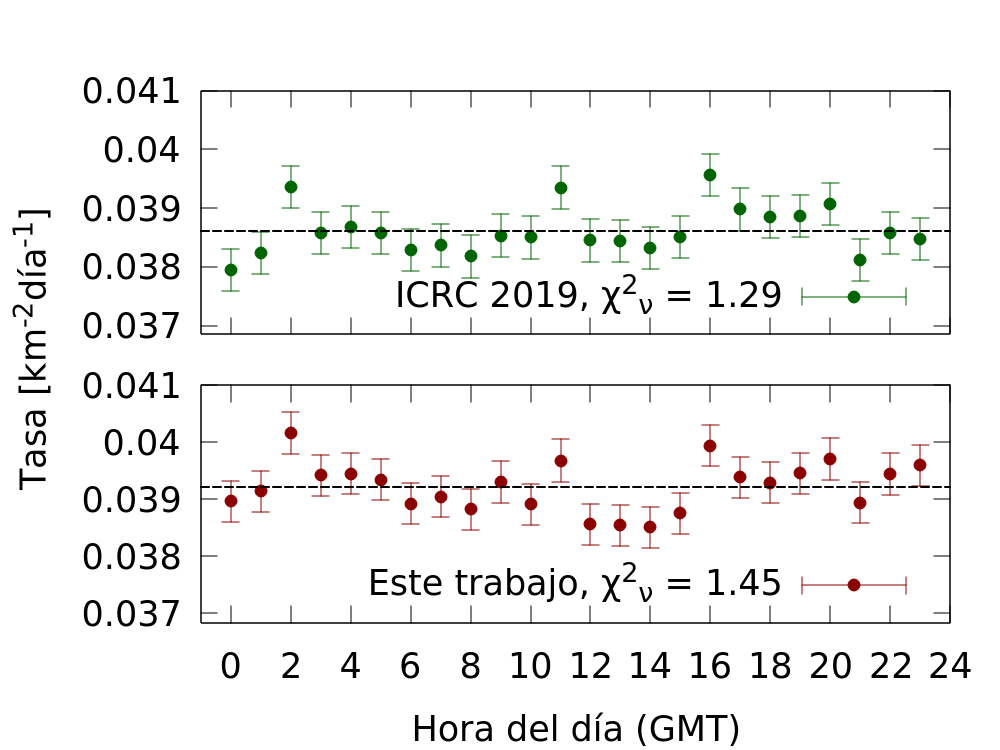
\includegraphics[width=\textwidth]{Graphs/2EeV_ICRC_2019_S38_S1000_expected.png}
                \caption{2005-2015} \label{fig:2EeV_expected}
                \end{subfigure}\\
                % \hspace{\fill}
                \begin{subfigure}[b]{0.5\textwidth}
                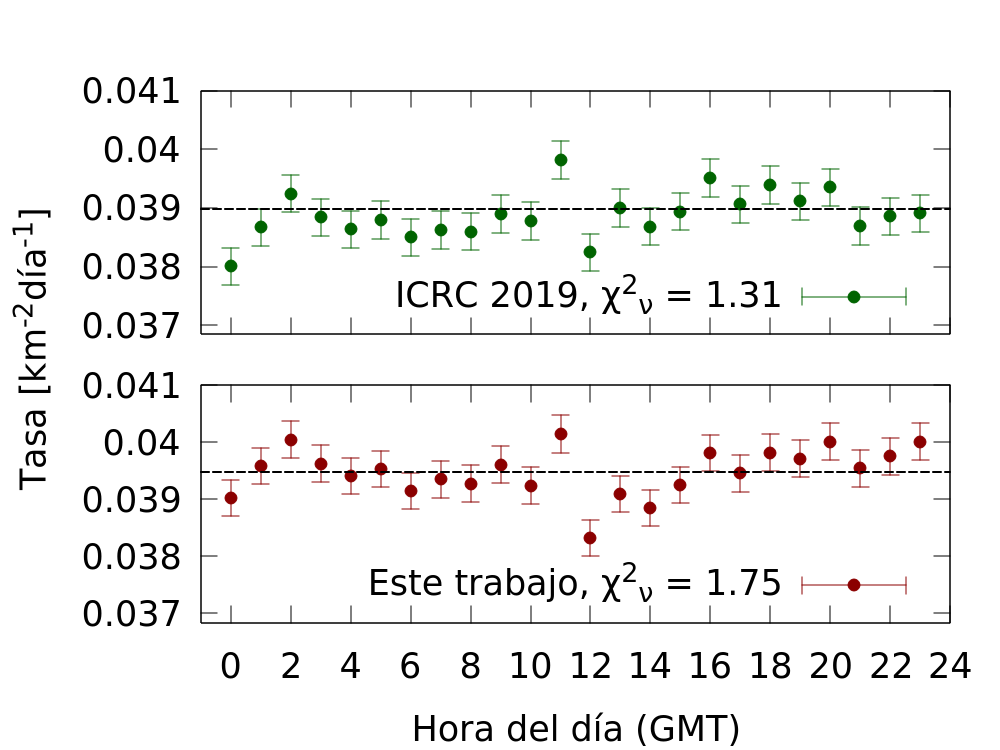
\includegraphics[width=\textwidth]{Graphs/2EeV_ICRC_2019_S38_S1000_expected_05_18.png}
                \caption{2005-2018}\label{fig:2EeV_expected_05_18}
                \end{subfigure}%
                \caption{Tasa de eventos por día para eventos de energía mayor a 2\,EeV para los datos de ICRC 2019 y la tasa de eventos obtenida con la reconstrucción de energía en este trabajo comparados en los periodos estudiados}\label{final}
        \end{figure}
Cabe aclarar que para la corrección de la energía para este trabajo, no se consideraron las posibles modulaciones de los valores del CIC o del posible cambio en los coeficientes de la Ec.\ref{eq:s38_energy}. Debido a que estos coeficientes son calibrados con eventos híbridos que son detectados durante la noche, donde las condiciones atmosféricas difieren de las condiciones promedios. Por ejemplo, en el caso de la densidad, durante la noche es aproximadamente $2\%$ mayor que el promedio.


\section{Eventos asociados a Todos los Disparos en el rango 2014-2020 }	\label{ALL_modulacion}
	

En esta sección se trabajó con el conjunto de datos registrados por el arreglo principal con Todos los Disparos. Las características de estos datos se resumen en la Tabla~\ref{tabla:caracteristicas_ALL} La señal de $S(1000)$ de este conjunto fue corregida en la reconstrucción oficial de eventos por la modulación del clima por los parámetros obtenidos en \cite{aab2017impact}.

\begin{table}[H]
  \centering
  \begin{tabular}{|c|c|}
  \hline
  Inicio              & 01  de Enero de 2014\\ \hline
  Final               & 01  de Enero de 2020       							\\ \hline
  Número de eventos   & 1\,263\,015							\\ \hline 
  Energía media       & 1.76\,EeV       				\\ \hline  %  1.005\,EeV
  Corte en $S_{38}$   & 5.36 VEM        				\\ \hline 
  Corte en ángulo cenital		  & $\theta < 60^o$ 				\\ \hline
  \end{tabular}
\caption{Características del conjunto de datos de Todos los Disparos.} \label{tabla:caracteristicas_ALL}
\end{table}



\begin{figure}[H]
  \centering
  \begin{subfigure}[b]{0.9\textwidth}
  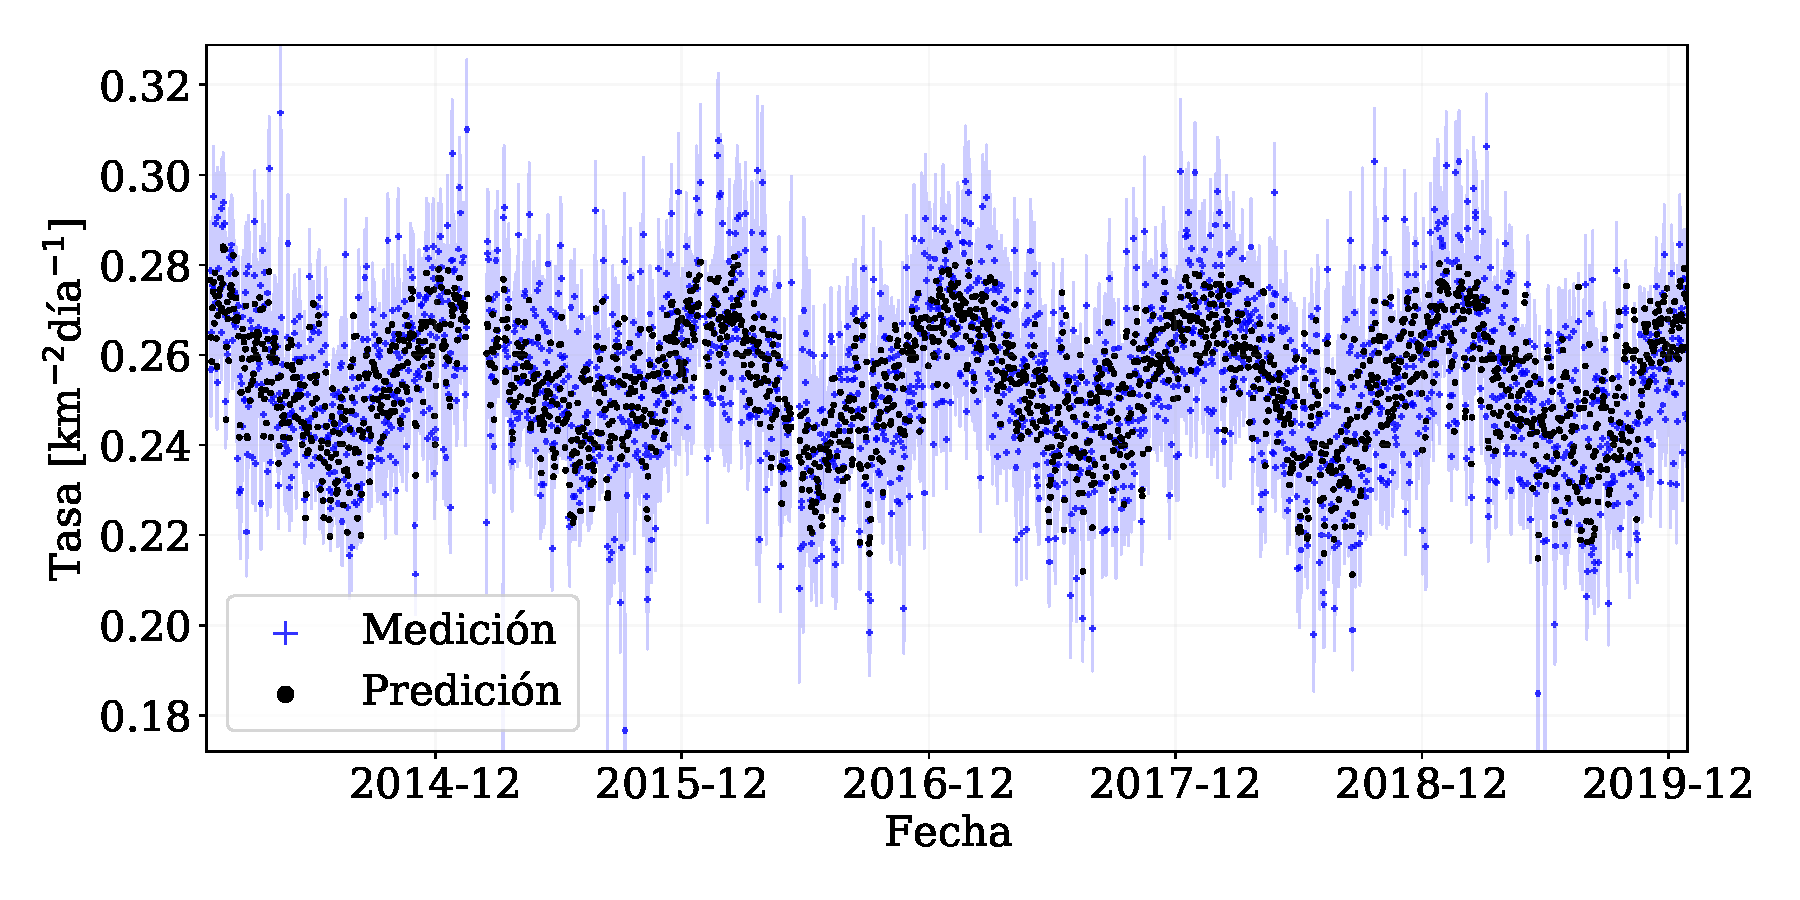
\includegraphics[width=\textwidth]{Graphs/rate_dayly/AllTriggers_S38_over_1EeV_rate_v3.pdf}
  \caption{Tasa eventos por día}\label{fig:rate_dayly_AllTriggers}
  \end{subfigure}\\
  \begin{subfigure}[b]{0.9\textwidth}
  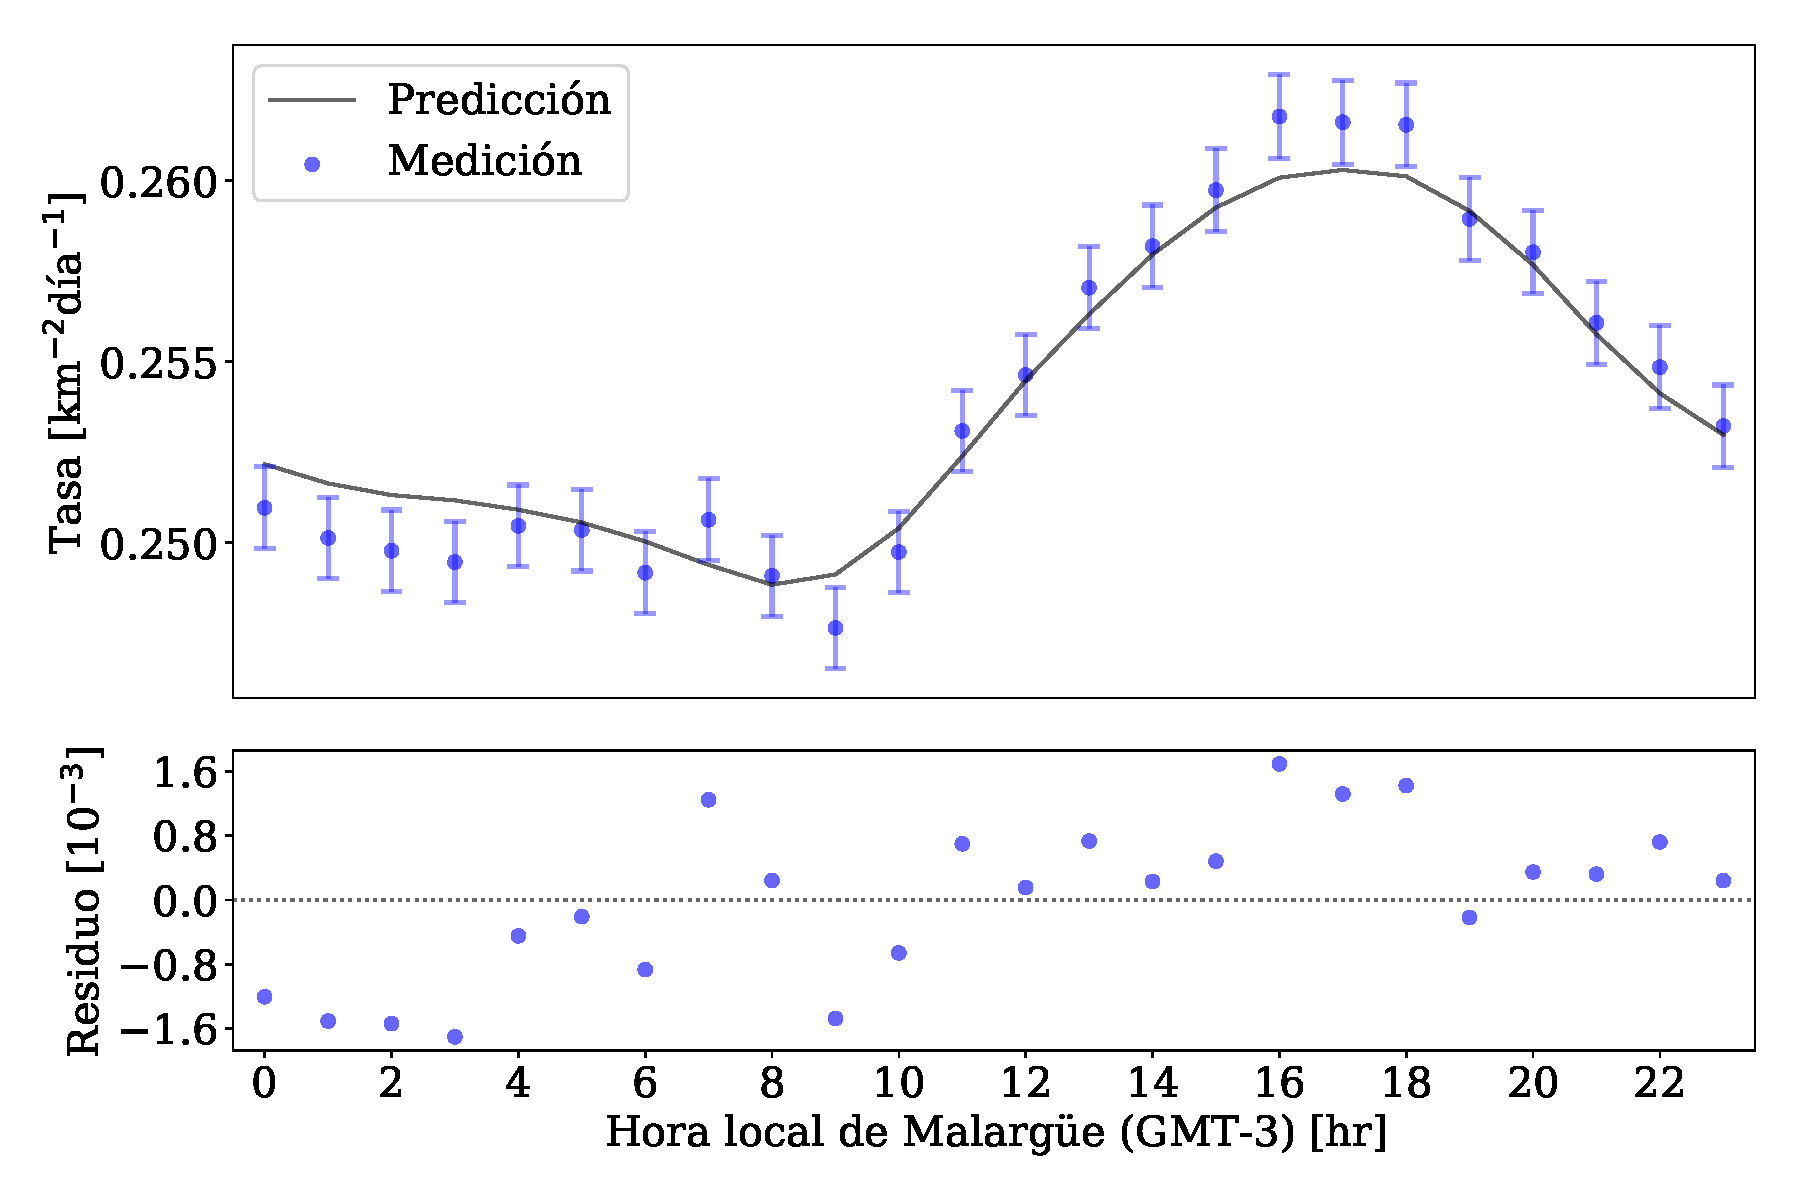
\includegraphics[width=\textwidth]{Graphs/rate_hour_of_the_day/AllTriggers_S38_over_1EeV_hour_of_the_day.pdf}
  \caption{Tasa de eventos promediada por hora del día }\label{fig:rate_hod_AllTriggers}
  \end{subfigure}
  \caption{Tasa de eventos por días comparadas con el ajuste entre los años 2014 hasta 2020. Estos eventos se registraron con Todos los Disparos  y tienen un valor de $S_{38,w}$ mayor a $5.36\,$VEM. En las tasas se observan la modulación anual y diaria del clima. }\label{fig:rate__AllTriggers}
\end{figure}

En este trabajo se busca comparar los parámetros obtenidos con los eventos de Todos los Disparos con los parámetros de la reconstrucción oficial. Para esto se realizó un análisis con los datos de nueva reconstrucción de la señal $S_{38}$ sin la corrección del clima, siguiendo un proceso similar a la sección \ref{sin_corregir_s38}.

% \subsection{Pesos de los hexágonos en el rango 2014-2020}

% Para constatar que no exista ninguna anomalía en los pesos de los hexágonos, se realiza el cálculo de los mismos para tres frecuencias de referencia para el análisis de anisotropías.  Los pesos se muestran en la Fig.\,\ref{fig:wei_14_20}. El rango de tiempo en el que se calculan estas curvas es entre 1 de Enero del 2014 y el 1 de Enero del 2020.

% \begin{figure}[H]
% 	\centering
% 	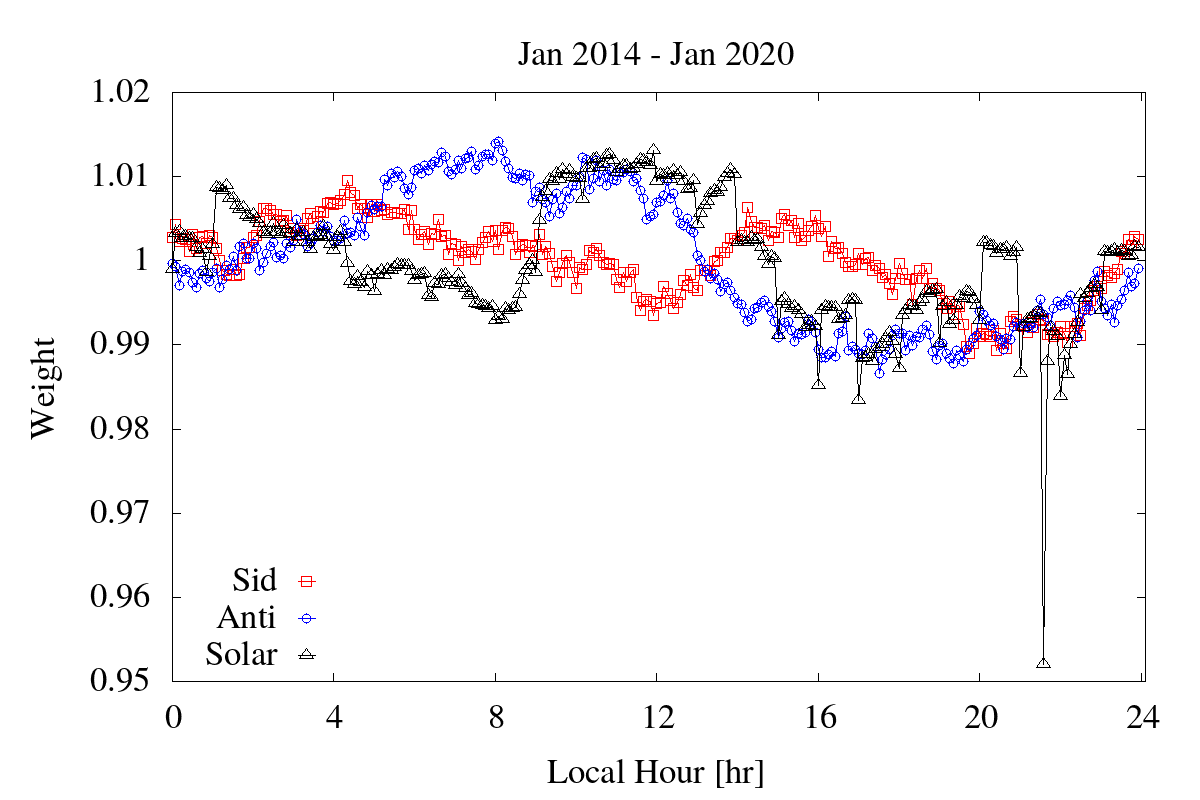
\includegraphics[width=0.5\textwidth]{weigth2014-2020_jan.png} 	
% 	\caption{Pesos de los hexágonos}
% 	\label{fig:wei_14_20}
% \end{figure}



      Considerando el filtro con el S38 en el archivo 2020 y la energía en el 2017, quiero saber si obtengo parámetros  del clima comparables. Ya que el Main Array se corresponden los parámetros del 2015 y 2019, yo esperaría que con todos los triggers pase los mismo. Una diferencia importante entre ambos análisis es que los parámetros del 2020 contienen eventos hasta el 31/12/2019.
      
      Los mismos se comparan con los ajustes obtenidos en \cite{aab2017impact}.

        \begin{figure}[H]
          \centering
          \begin{subfigure}[b]{0.8\textwidth}
          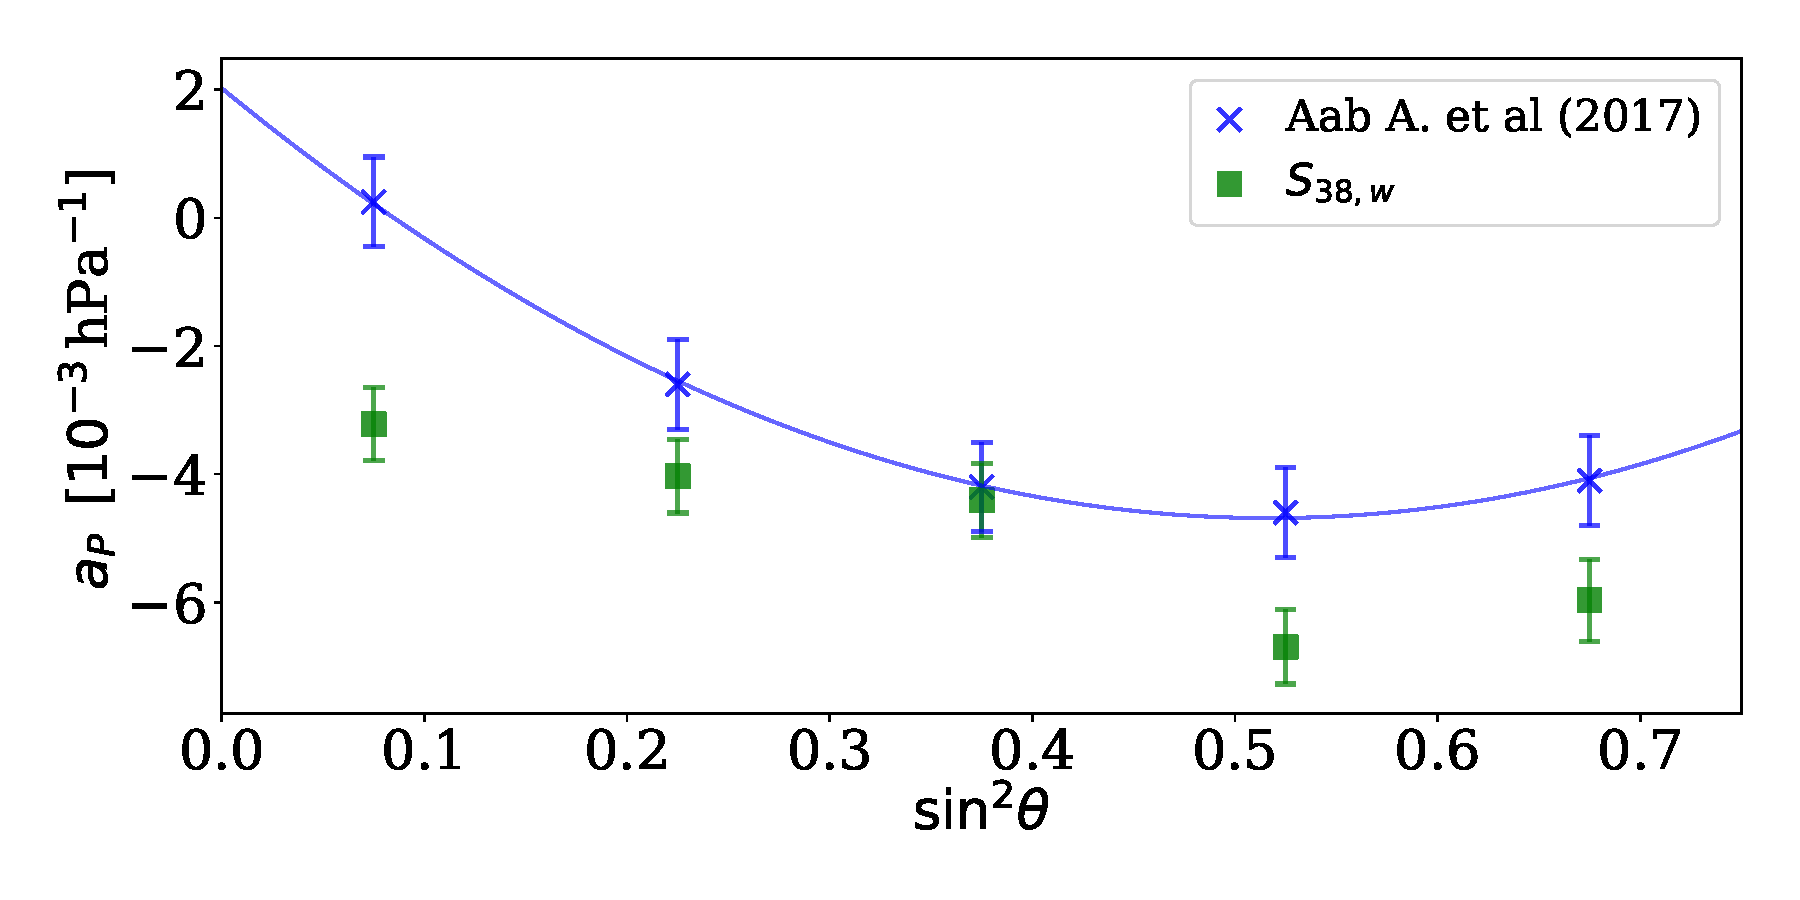
\includegraphics[width=\linewidth]{Graphs/params/ap_AllTriggers.pdf}
          \caption{Parámetro $a_P$ }
          \end{subfigure}\\
          \begin{subfigure}[b]{0.8\textwidth}
          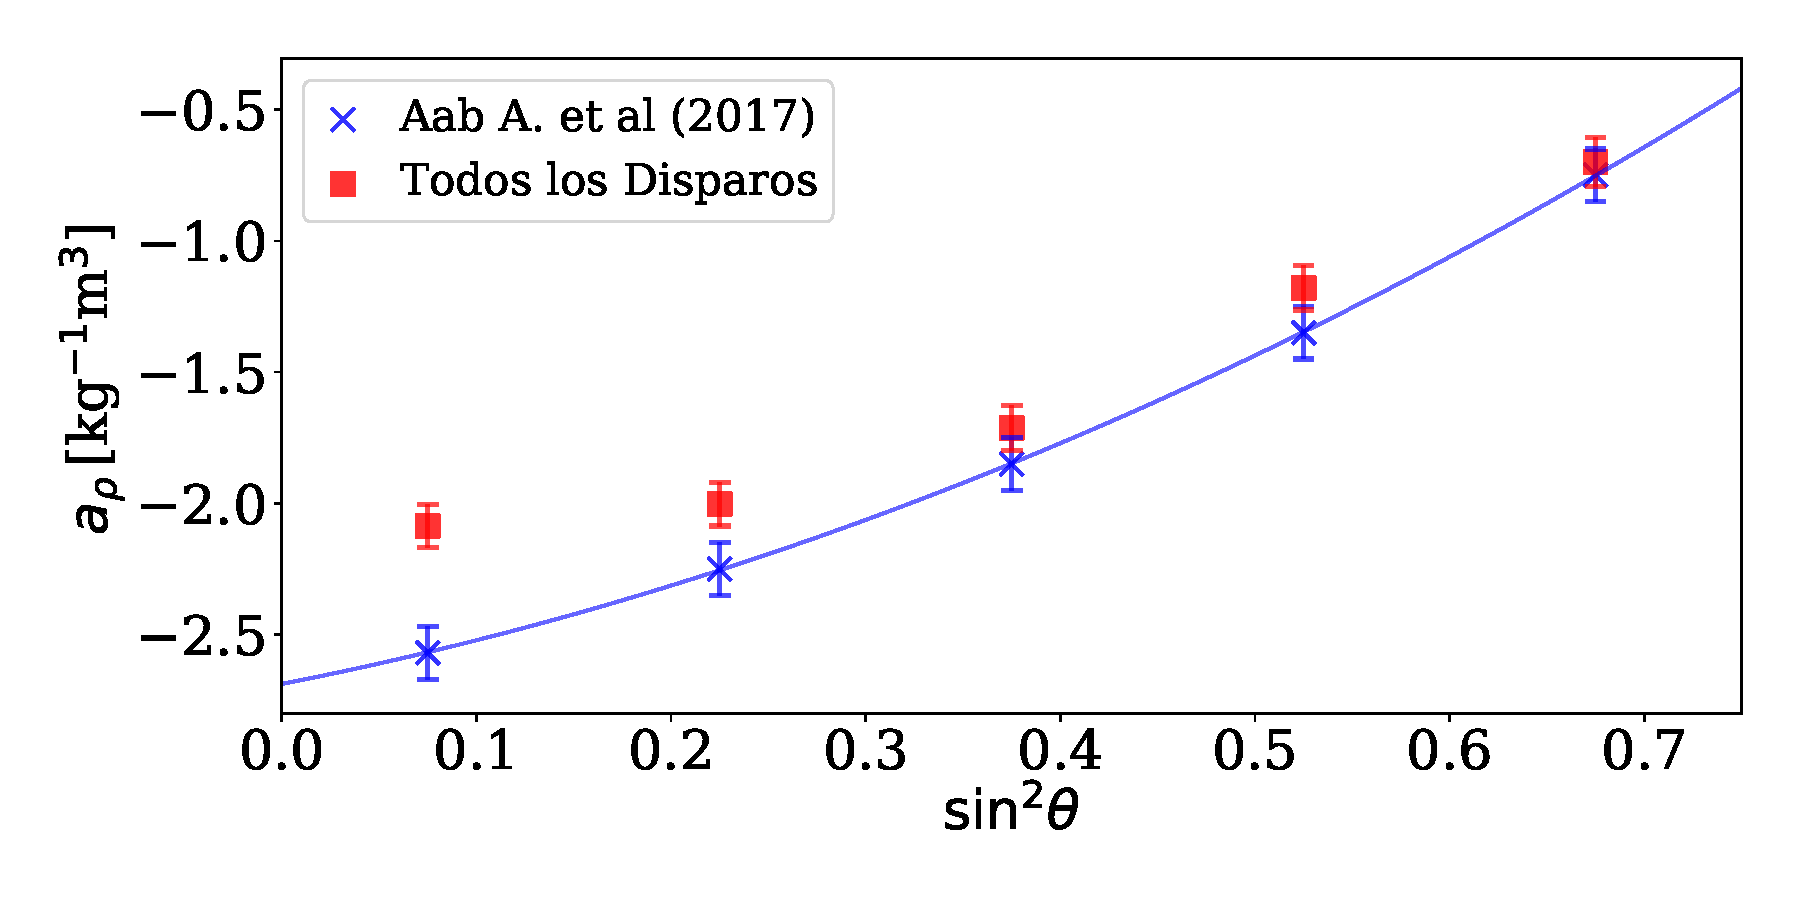
\includegraphics[width=\linewidth]{Graphs/params/arho_AllTriggers.pdf}
          \caption{Parámetro $a_{\rho}$ }
          \end{subfigure}\\
          \begin{subfigure}[b]{\textwidth}
          \centering
          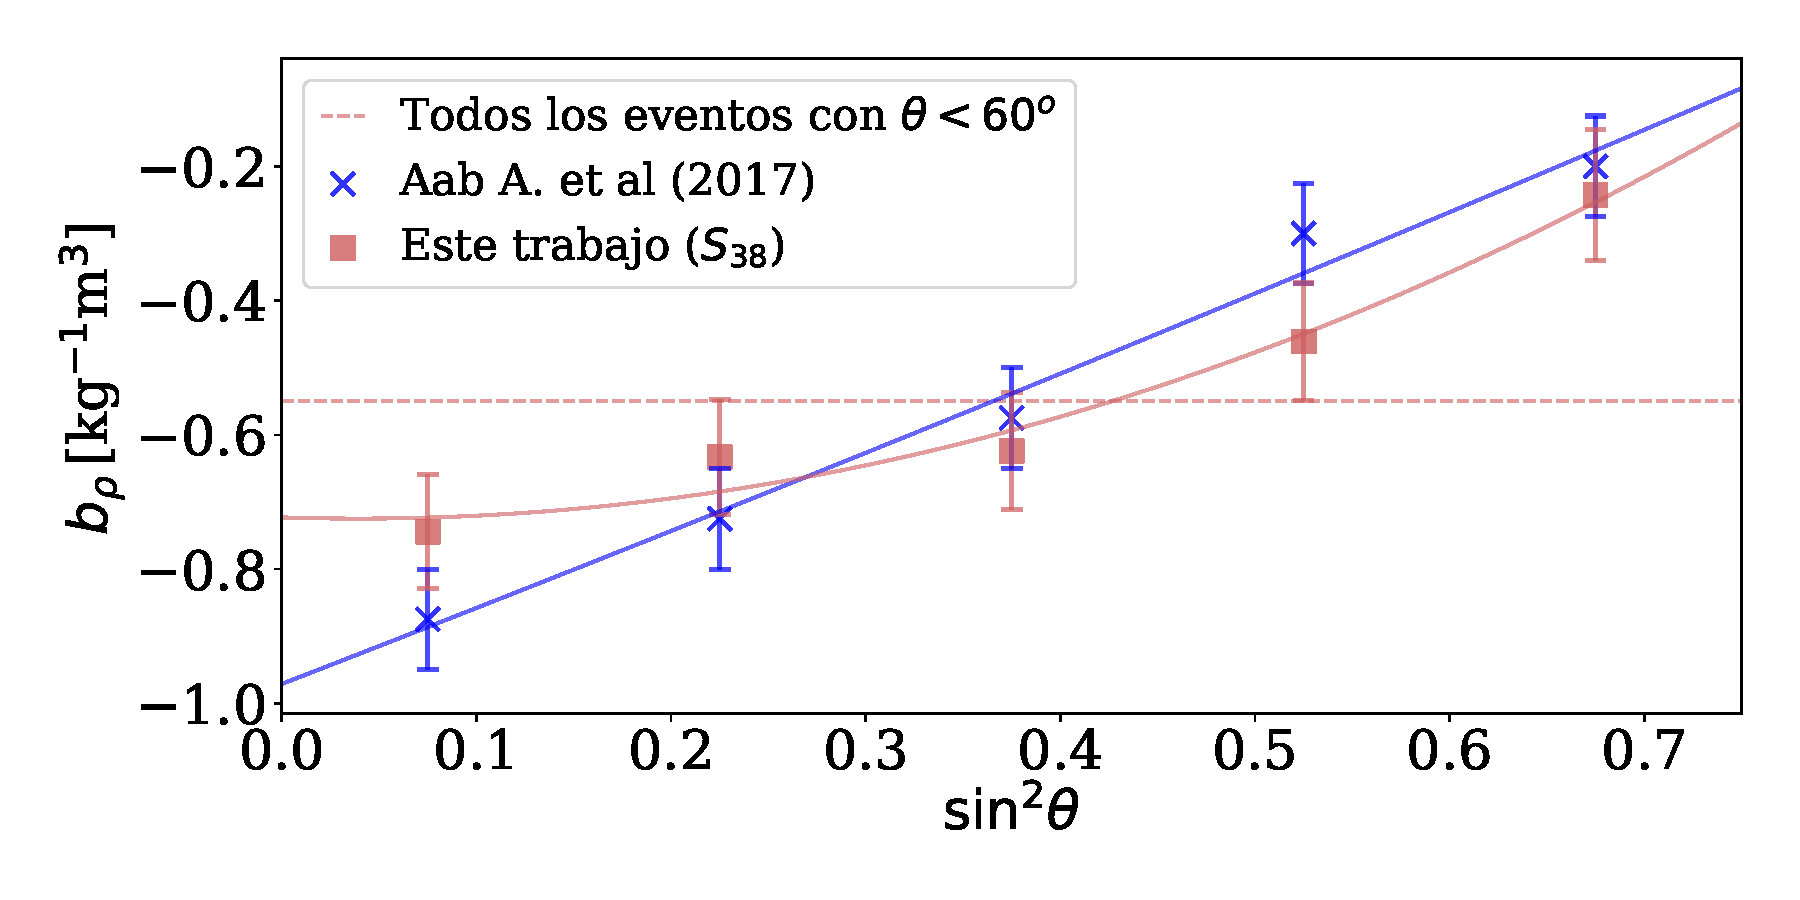
\includegraphics[width=0.8\linewidth]{Graphs/params/brho_AllTriggers.pdf}
          \caption{Parámetro  $b_\rho$   }
          \end{subfigure}
          \caption{Parámetros de la modulación del clima considerando los datos para todos los disparos del archivo 2017 y 2020. Los mismos se comparan con los coeficientes utilizados por la Colaboración.}
        \end{figure}

%       ???????????Se ve que estos parámetros no son comparables. 
